\documentclass[output=paper]{langscibook}
\ChapterDOI{10.5281/zenodo.18845926}
\author{Virve-Anneli Vihman\orcid{}\affiliation{University of Tartu, Estonia} and Mari-Liis Korkus\orcid{}\affiliation{University of Tartu, Estonia} and Maarja-Liisa Pilvik\orcid{}\affiliation{University of Tartu, Estonia} and Kristiina Praakli\orcid{}\affiliation{University of Tartu, Estonia}}
\title[The integration of English in Estonian teenagers’ instant messages]{\textit{Verinaiss} ‘very nice’:  The integration of English in Estonian teenagers’ instant messages}
\abstract{This paper analyzes Estonian teenagers’ code-switching with L2 English in instant messaging (IM) language. We focus on the orthographic and morphological integration of English units and consider the variability inherent to the IM register. The analysis is based on the newly compiled Corpus of Estonian Teenagers’ Language, containing spoken and IM language from informants aged 10--18; for this study, we analyze the IM conversations, containing 60,000 words from 102 informants, 99 of whom use at least some English. On average, 7.5\% of words are in English, with great fluctuation between speakers and conversations.

Our data support the gradient view of morphosyntactic integration expressed by \citet{Deuchar2020}. It has been shown that IM chat language deploys strategies imitating spoken and written language, as well as bearing features distinguishing it from both: code-switching in the IM register also shows features unlike either spoken or written registers, including the variability in orthographic integration. Our data show how Estonian teenagers make ample use of their L2 English in conversations with other Estonian teens, as an extension of their Estonian language usage. Orthographic integration is optional, playful, and sometimes serves to flag unintegrated phonology. Morphological integration is more fundamental to language fluency, and we find that over 80\% of nouns and verbs in contexts requiring morphological marking are marked, whereas adjectives are much less likely to be marked. Despite the register’s preference for unconventional usage, code-switching in our data follows the expectations based on spoken-language code-switching more often than it flouts them.

\keywords{Youth language, instant messaging, corpus linguistics, code-switching, Estonian}
}
\IfFileExists{../localcommands.tex}{
  \addbibresource{../localbibliography.bib}
  \usepackage{tabularx,multicol}
\usepackage{url}
\urlstyle{same}

 
\usepackage{langsci-optional}
\usepackage{langsci-lgr}
\usepackage{langsci-gb4e}

\usepackage{multirow}
\usepackage{cleveref}
\usepackage{subfigure}
\usepackage{langsci-branding}

  \input{../localcommands} 
  \input{../localhyphenation} 
  \togglepaper[3]%%chapternumber
}{}

\begin{document}
\maketitle 
%\shorttitlerunninghead{}%%use this for an abridged title in the page headers
% ATTENTION: Diacritics on the following phonetic characters might have been lost during conversion: {'ɪ'}

\section{Introduction}

Teens are considered to be innovative language users and potential initiators of language change (\citealt{Cheshire2005, Leppänen2007}). Eckert’s depiction of teenagers as linguistic “movers and shakers” (\citealt{Eckert1997}: 52) refers to their creativity and use of linguistic resources to create new linguistic practices, identities, and values (see \citealt{StenstromEtAl2002, Nortier2018}). The continual emergence of new linguistic practices is witnessed in today’s digitally mediated conversations, where the diverse linguistic, cultural, and audiovisual resources and the endless stream of “content” provides a wealth of opportunity for communicative creativity and innovation. Additionally, the online environment experienced by teens in many parts of the world includes a blend of languages, fostering \textsc{polylingualism} \citep{Jørgensen2008} and \textsc{translanguaging} (\citealt{García2009, GarciaWei2014}), both of which include the idea that multilingual language use does not require language fluency, noting that any linguistic resources can be drawn upon in a communicative context to varying effects.

While teenagers’ language use has been described as a distinct \textsc{code} or \textsc{register} (see \citealt{Androutsopoulos2005, Tagliamonte2016teen}), those teenagers inhabiting a multilingual environment raise intriguing questions for researchers regarding innovation, variation, and the use of linguistic resources for negotiating social identity. The ‘translanguaging’ in linguistic practices among young people in urban spaces differs from what has been traditionally examined in multilingualism and code-switching research, both in the language backgrounds of the speakers and in their language usage. This approach ascribes dynamic fluidity to the speakers, who make use of their entire linguistic repertoire and competencies to express themselves. In addition to studies which have focused on English-speaking teenagers, previous studies have described youth registers in the context of other languages including Swedish \citep{Kotsinas2004}, Danish \citep{Quist2010}, Dutch (\citealt{SchoonenAppel2005}), Belgian Dutch or Flemish (\citealt{SchuringZenner2022}), and Spanish \citep{Jørgensen2013}. Earlier studies have mostly focused on spoken language, but researchers have emphasized the need for more research on computer-mediated communication (e.g., \citealt{Quist2010}: 10).

In this paper, we investigate the language used in instant messaging (IM) by Estonian teenagers who inhabit a multilingual media environment despite the relatively monolingual character of their offline environments. In the context of today’s social interaction, IM exchanged on digital devices has taken the place of much spoken conversation and are key to understanding the communicative and social behavior of contemporary youth (\citealt{TagliamonteDenis2008, Tagliamonte2016sick}). IM conversations include a vast array of visual, textual, and intertextual options for conveying both meaning and affect: teenagers’ communication reflects a polyphonic, multimodal discourse in which they navigate seamlessly. Among these multiple layers is their use of multiple languages. The Estonian teens draw on Estonian and English, with varying amounts of Russian as well, using twice as much English when they chat online with each other than in their spoken conversations (\citealt{VihmanEtAl2022}; cf. \citealt{Androutsopoulos2005}). As such, they embody the recent phenomenon of “networked multilinguals” \citep{Androutsopoulos2015}, online communicators whose experience with English may be minimal offline, but who embrace a multilingual mode of communication online. How the languages are combined in this “third register” – differing from both written and spoken language – requires empirical investigation, as it sheds light on the current generation of youth residing in a mediatized and globalized communicative space. The research that has investigated multilingual youth in this context has mostly focused on migrants. Here, we focus on youth who have become multilingual in large part through the use of globalized media.

In this study, we investigate how Estonian adolescents use English linguistic elements – by far the most frequent non-Estonian insertions – in the context of online social interaction among Estonian-speaking friends. This indicates whether they conceive of their conversation structure as following the frame of a single language or not (e.g., \citealt{Myers-Scotton2006}). We employ combined quantitative and qualitative analysis of multilingual practices in the IM conversations of Estonian teenagers, focusing on two research questions: To what extent and in what ways are English elements integrated into (primarily) Estonian conversations orthographically? And to what extent and in what ways are they integrated morphologically? The data derive from the Teen Speak in Estonia chat corpus,\footnote{“Teen Speak in Estonia” project: \href{http://www.sisu.ut.ee/teke}{www.sisu.ut.ee/teke} (02 May, 2023).} containing 109 IM conversations between 102 unique participants aged 10 to 18. 

Because Estonian spelling is phonetically transparent and hence is taken by speakers to directly indicate pronunciation, the orthographic renditions of words in the informal register of IM can be played with to indicate phonological (non-)integration of linguistic units into the matrix code. We ask whether the teenagers in our study make systematic use of orthographic integration (Estonianized spelling) to indicate phonological integration (indicating Estonianized pronunciation), and whether orthographic and morphological integration are correlated in the same way that has been found for phonological integration between English and Spanish (\citealt{Bessett2017}; see also discussion in \citealt{Deuchar2020}). Orthographic integration is variable, as shown in \textit{verinaiss} ‘very nice’ compared with the unintegrated \textit{verygood} (both attested in the corpus); variants of ‘thank you’ – e.g., \textit{tänk ju} (see \sectref{sec:vihmanetal:4.2.1}) – can be taken to clearly evoke pronunciation as well. These questions are important both for understanding the way the participants deploy their multilingualism for constructing meaning and identity, but also for research into code-switching. The relationship between integration in morphology and phonology has long been discussed (e.g., \citealt{Poplack1980}), but the relation between phonological and orthographic integration may take on a new significance in IM chats, which are able to – but not compelled to – mimic pronunciation.

The spontaneity of the IM context is expected to facilitate a range of solutions to the question of morphological integration. While various structural and social constraints on code-switching have been outlined in the literature on multilingual spoken conversation (e.g., \citealt{Myers-Scotton2006}), the IM context is one in which speakers are likely to defy both constraints and norms in the interest of ease of production and to maintain a certain breeziness that is characteristic of the format. As discussed in relation to Russian and Estonian by \citet{Verschik2007,Verschik2016} and \citet{ZabrodskajaVerschik2014}, morphological and phonological integration need not be interdependent; each depends to a large part on individual preference and cannot be predicted solely based on structural compatibility, particularly in computer-mediated communication, in which spontaneity and great variability are prevalent.

In the following section, we discuss relevant background context, describing characteristics of IM, Estonian-English contact in light of youth language and young people’s internet usage, and morphosyntactic and orthographical aspects of the Estonian language crucial to the analysis. In \sectref{sec:vihmanetal:3}, we describe the data and method used for this study. In \sectref{sec:vihmanetal:4}, we present the results of the analysis, describing in more detail how English elements are integrated orthographically and morphologically in Estonian chat conversations. We conclude with a discussion and concluding remarks.

\section{Background}\label{sec:vihmanetal:2}
\subsection{Language used in instant messaging}

Much of today’s communication occurs in online spaces (e.g., social media and instant messaging applications; see \citealt{ThurlowMroczek2011}), shaped alongside rapid technological developments in the past twenty to thirty years. Both the availability of these online written formats and their technical constraints have affected language use to the point where a new language register or variant has been identified across various languages (\citealt{CollotBelmore1996, Androutsopoulos2014, McCulloch2019}). Proposed labels for this new type of language include netspeak, chat language, internet slang, web-based language, internet language, or, perhaps most commonly, \textsc{computer-mediated} \textsc{communication} (CMC; see \citealt{Herring1996, Crystal2001, Androutsopoulos2006}). 

While CMC describes the language used in technologically mediated discourse (\citealt{AndroutsopoulosEtAl2013, Vettorel2014}), it is a broad umbrella term, referring to various web-based communicative practices, including not only spontaneous texted communication but also edited contexts like blogs, vlogs, and forums more generally. In this paper, we focus on a synchronous language variant used in communication between two or more speakers in rapid messaging applications (particularly Facebook Messenger and Discord), and we refer to it as \textsc{instant} \textsc{messaging} (IM) \textsc{language} (see \citealt{Herring2007, TagliamonteDenis2008, Baron2010}).

IM language combines numerous features from written and spoken language while adapting to the technological capabilities of online spaces (e.g.,   \citealt{PalfreymanAlKhalil2003}) and the orthographic affordances of the written format. One frequent feature involves using abbreviations and short forms (cf. \citealt{ThurlowBrown2003, TagliamonteDenis2008}), such as \textit{wdym} for ‘what do you mean’ and \textit{k} for ‘okay’. The technical limitations of earlier mobile device models directly influenced this characteristic: writing a text message or \textsc{SMS} (\citealt{HardAfSegerstad2005, Ling2005}) was time-consuming, limited in length, and costly; consequently, users found innovative ways to write messages more concisely \citep{Crystal2009}. Although current texting applications no longer have these character limitations and allow more character variety, message shortening is still frequent. This can be partially attributed to the speed of typing a message and partially to the distinctive language register, co-creating and enacting a shared knowledge of the abbreviations’ meanings \citep{Tagliamonte2016sick}.

Signs of creativity and experimentation are especially evident in IM typography (\citealt{VarnhagenEtAl2010, Herring2022}). The use of upper- and lowercase letters functions similarly to prosody in spoken language: they allow the user to emphasize a message (e.g., with UPPERCASE letters often interpreted as shouting, or having an intensified meaning) or give it a specific undertone (with lowercase writings used for aesthetics or aLtErNaTiNg CaPs for expressing playfulness). Along with text capitalization, IM users employ repeated letters to echo (but not necessarily mimic) lengthened pronunciation or emphasis (e.g., \textit{pleeeease}, \textit{omggggg} ‘oh my god’, \textit{nopeee} ‘nope’), as well as punctuation marks (e.g., repeated exclamation marks to express strong emotion) and what are known as keyboard smashes (e.g., \textit{asdfghjkl}; see \citealt{McCulloch2019}: 6) for emphatic or emotional effect. While gestures and facial expressions contribute to meaning-making in spoken interaction, various visual components in IM language function in a similar way. \citet{GawneMcCulloch2019} describe emoticons, emojis, and animated GIFs as \textit{digital gestures}. Depending on the context, these can accompany a written text or hold meaning independently. 

As literary practices have adapted to online spaces, so have the languages – and specifically orthographies – in which IM (and other web-based) texts are produced. One example of this adaptation is the process of \textsc{trans-scripting} \citep{Androutsopoulos2020}, where a language is respelled with alternative characters, reflecting a type of orthographic integration. Trans-scripting is often employed with languages that make use of a non-Latin script (e.g., \citealt{Su2003, Androutsopoulos2012}); however, we can observe this kind of adaptation in languages where the spelling reflects pronunciation, e.g., the word ‘nice’ written as \textit{naiss} in Estonian. 

Another distinguishing feature of IM involves the representation of colloquial, spoken language in the spelling conventions, such as \textit{dunno} for ‘I don’t know’ and \textit{prolly} for ‘probably’ in English. In Estonian, spelling more directly reflects the phonetic system (see \sectref{sec:vihmanetal:2.3}) and can easily be deployed to indicate the phonetic modifications arising in rapid speech. Specific, pronunciation-based variants have come into everyday use as IM usage has spread, including frequent collocations like \textit{see on} ‘this is’ > \textit{sen, ma olen} ‘I am’ > \textit{malen,} \textit{ma ei tea} ‘I don’t know’ > \textit{mtea, mdea}. Other commonly used pronunciation spellings include \textit{põmst} (< \textit{põhimõtteliselt} ‘basically’), \textit{tegelt} (< \textit{tegelikult} ‘actually’), and \textit{aint} (< \textit{ainult} ‘only’).

In interactions among multilingual interlocutors, \textsc{code-switching} is frequent. Known as the alternation of two languages (or language variants) within a single discourse \citep{Poplack1980}, code-switching can occur both intra- and intersententially. As noted earlier, the polylingualism characteristic of IM language puts the very notion of code-switching into question, as it is not always clear whether the speaker is “switching” between languages or making use of an emergent language blend. Most of the research on code-switching examines data collected from spoken language, while research on multilingual language use in the context of computer-mediated communication is in its early stages. \citet{Deuchar2020} notes that even in spoken discourse, differentiating between a code-switched or borrowed element is less than straightforward (we explain how we tackled this in \sectref{sec:vihmanetal:3.2}). The inherent variability of code-switching (or polylanguaging) in IM practices further complicates the question. \citet{Barasa2016}, investigating code-switching in Kenyan university students’ online messages, concludes that CMC code-switching should be treated as distinct from spoken code-switching, as certain discourse functions were identified as unique to CMC. Others investigating the pragmatic functions of code-switching have arrived at the same conclusion (\citealt{Hinrichs2006, Herring2013}). \citet{Androutsopoulos2015} further expands this theorizing by proposing the term \textsc{networked} \textsc{multilingualism} to describe the multilingual practices in and characteristic to social network environments. A major focus of studies concerning CMC-centered multilingualism is the use of English (and its adaptation) in the context of other languages.  \Citet{DeDeckerVandekerckhove2012} investigated the use of English in the MSN conversations of Flemish adolescents; \citet{Isenmann2022} observed the use of English in Icelandic Facebook;  \citet{VerheijenVanHout2022} examined social media messages of Dutch youth. All these studies report that both the use and integration of English lexical items is highly variable, with the elements (particularly phrases and longer units) sometimes remaining unadapted, while in other cases English is creatively integrated within the graphemic and morphological frames of the matrix language. The localization of English shows that CMC-centered multilingual practices should be fruitfully viewed as a form of translanguaging.

\subsection{Estonian-English contact, youth language and the internet}

The last three decades have crucially brought about two types of language contact in Estonia (\citealt{PraakliKoreinik2020}): first, the number of languages in contact with Estonian has doubled since the country regained independence in 1991; secondly, contact between Estonian and English speakers has greatly increased. English is used as a common language with people of varying backgrounds and in online communication. English-Estonian contact is more multifaceted than it was in the past when it was mostly characterized by cultural loanwords and translations (\citealt{Jogi2014}). English functions as the international lingua franca in politics, business, and entertainment. In some situations, English is used as a vehicular language, while in others, it is drawn on as an additional communicative resource to serve various discursive purposes (\citealt{Kask2021, PraakliEtAl2022, VihmanEtAl2022}).

The latest census (\citealt{Statistics2022population}) reported that 48\% of the population spoke English as a foreign language, making it the most widely spoken foreign language in Estonia. In the period since previous censuses (2000, 2011), the presence of English in Estonia has grown steadily. However, English proficiency varies considerably by age; it is highest among adolescents and young adults, with 85\% of 15- to 29-year-olds claiming to speak English as a foreign language (\citealt{Statistics2022demographics}). English is now taught as the first compulsory foreign language at school. The EF English Proficiency Index \citet{Education2022} highlights Estonians’ high English language proficiency, especially among young people.

The internet and other rapidly developing technology of recent decades have opened up unlimited access to English-language networks and media content. Most children in Estonia are exposed to English via media from an early age. \citet[1027]{KalmusEtAl2022} remark that the past decade has seen significant changes in how the internet and digital devices influence the lives of children and youth, such as a substantial increase in the proportion of smartphone-using children and the amount of time they spend online each day, watching videos on YouTube or social networking on global platforms such as Instagram, TikTok, and WhatsApp. Estonian children’s internet use has increased markedly, with 97\% of children aged 9--17 accessing the internet every day in 2018, compared to 82\% in 2010 (\citealt{SukkSoo2019}; similar statistics are reported by \citealt{KalmusEtAl2022}: 1033). The media practices of young Estonians are increasingly multilingual, with English holding a key position \citep{PraakliEtAl2022}. The use of English alongside Estonian reflects their changing linguistic habits, contexts of use, and sources of linguistic input. Although Estonian teenagers acquire English at school, the term \textsc{foreign} \textsc{language} is not adequate for defining the position of English in their lives. Beyond classes at school, English is acquired through the internet and entertainment. The effects of English as a global language are noticeable in countries like Estonia, where (a) the relatively small population means that the production of entertainment in the national language is much more limited than in English, particularly regarding entertainment targeted at teenagers, and (b) liberal social attitudes mean that young people are given a great deal of autonomy in organizing their extracurricular time.

Hence, for today’s Estonian teenagers, English is neither the L1 (first language) nor a foreign language (learned outside the environment in which it is spoken). It would be appropriate to describe it as a \textsc{second} \textsc{language} (L2) learned partly through \textsc{immersion}, despite the virtual nature of that immersion. Teenagers are digital natives who converse even with their local friends mostly through instant messaging, social media, and smart devices (see \citealt{Paus-HasebrinkEtAl2019}). Although the English-language input in the immersion context is mostly virtual, for this generation, that is a seamless extension of their ordinary language use and a fairly natural context of acquisition, as well as an organic enhancement of their interactions with their peers: although a group of friends may be all L1 Estonian speakers, they will draw on English when communicating with each other because of their shared polylingual online experiences. We note that today’s teenagers often feel at home in their L2 English, switching easily between Estonian and English.

In summary: the multilingualism of this generation should not be understood as “full competence in different languages” (\citealt{BlommaertEtAl2005}: 199), but as a core feature of their language use and communicative needs (see \sectref{sec:vihmanetal:3} for participants’ proficiency). In young people’s spontaneous spoken conversations \citep{VihmanEtAl2022}, computer-mediated interactions (\citealt{Igav2013, Kilp2021}), and performative videos \citep{PraakliEtAl2022}, English functions as an additional language resource, used for stylistic and pragmatic purposes. Nevertheless, data on the role of English in unedited, spontaneous, digitally mediated discourse among young people in Estonia is sparse.

\subsection{Some features of Estonian morphosyntax and orthography}\label{sec:vihmanetal:2.3}

\begin{table}[b]
\begin{tabularx}{\textwidth}{XXXlll}
\lsptoprule
 &  {\textsc{nom.} \textbf{sg}} &  {\textsc{gen.sg}} &  {\textsc{par.sg}} &  {\textsc{all.sg}} &  {\textsc{nom.pl}}\\
 \midrule
apple & \textit{õun} & \textit{õuna} & \textit{{\textasciigrave}õuna} & \textit{õuna-le} & \textit{õuna-d}\\
swing & \textit{kiik} & \textit{kiige} & \textit{kiike} & \textit{kiige-le} & \textit{kiige-d}\\
chair & \textit{tool} & \textit{tooli} & \textit{{\textasciigrave}tooli} & \textit{tooli-le} & \textit{tooli-d}\\
book & \textit{raamat} & \textit{raamatu} & \textit{raamatu-t} & \textit{raamatu-le} & \textit{raamatu-d}\\
family & \textit{pere} & \textit{pere} & \textit{pere-t} & \textit{pere-le} & \textit{pere-d}\\
\lspbottomrule
\end{tabularx}
\caption{Partial inflectional paradigms for Estonian nouns: five example lexemes, five paradigm cells (Nominative, Genitive, Partitive and Allative singular; Nominative plural)}
\label{tab:vihmanetal:1}
\end{table}


Estonian is a Finno-Ugric language affected by contact with Indo-European, especially German and Russian, but genetically unrelated to English \citep{Metslang2009}. Whereas English is analytic and employs rigid word order to indicate grammatical structure, Estonian is fusional-agglutinative and makes rich use of inflectional morphology for marking grammatical relations and argument structure. 

Estonian nouns take fourteen cases in singular and plural, while in English, only pronouns show any case-marking. Plurals are marked in both languages. English plurals are generally marked with an -\textit{s}, though irregular plurals have various patterns. Estonian nominative plurals are marked with a regular -\textit{d} affix, which is attached to the genitive stem rather than the nominative (see \tabref{tab:vihmanetal:1}, final column). Importantly, the genitive always ends in a vowel, known as a \textsc{theme} \textsc{vowel} (glossed as \textsc{tv),} but which particular vowel (\textit{a}, \textit{e}, \textit{i}, or \textit{u}) is lexically specified (\tabref{tab:vihmanetal:1} gives examples of genitive formation). Nouns ending in a vowel in the nominative case (e.g., \textit{pere} in \tabref{tab:vihmanetal:1}) often use the same form in genitive singular. Importantly, the genitive form acts as a stem for the nominative plural and most of the singular cases (e.g., allative in \tabref{tab:vihmanetal:1}), and the vowel is crucial for the phonotactics of adding the case suffixes.

Partitive case, which is used to mark direct objects as well as partitivity, is formed in two ways in the singular across different declension classes, with either vowel-final forms (\textit{õuna}, \textit{kiike}, \textit{tooli} in \tabref{tab:vihmanetal:1}) or forms ending in -\textit{t/d} (\textit{raamatut}, \textit{peret}). Genitives and vowel partitives may involve stem changes.

Estonian verbal morphology is agglutinative and, as in noun morphology, the stem ends in a vowel. Verb affixes mark tense, person, number, mood, and voice in their finite form or receive various infinitival markers.

The wealth of inflectional morphology used in Estonian requires speakers to make frequent choices with borrowings and code-switched words, to (a) mark them with morphology from the source language, (b) mark them with morphology from the matrix language, or (c) leave them unmarked. \citet{Zabrodskaja2009} describes the gradience of morphological integration for Estonian words used in Russian (see also discussion in \citealt{Vihman2016, Kask2019}), including the question of whether or not morphology is required but also various intermediate levels between no integration and full integration. In Estonian, morphological marking involves further choices, notably how to accommodate stem changes on elements from other languages and which theme vowel to use with grammatical affixes. Because of the mixture of stem-changing and affixal morphology, integration into Estonian allows for differing degrees of integration, similar to what was described for Welsh by \citet{Deuchar2020}.

For neologisms, loanwords, or switches integrated into Estonian morphology, the default theme vowel is -\textit{i}, used for both nouns and verbs. English orthography often provides another alternative: although the unpronounced -\textit{e} found at the end of many words (e.g., \textit{nice}, \textit{smile}) does not affect phonological integration in the spoken language, it can influence how speakers accommodate inserted stems in informal written code-switching. 

The two languages also differ in their orthography. Unlike English, which uses an opaque writing system, the orthography of Estonian is essentially phonetic. Phonemes are transparently mapped to letters, with a nearly one-to-one correspondence. The Estonian alphabet includes four vowels with diacritics, Õ pronounced /ɤ/, Ä /æ/, Ö /ø/ and Ü /y/. The letters C, Q, W, X, Y, and Z are only used in loanwords, foreign names or playful spellings. Y has often been used informally instead of Ü to denote /y/, as it is used in the closely related Finnish language. The Y used in English words can be \textsc{estonianized} with various representations: J (e.g., \textit{jess} for ‘yes’), AI (\textit{oomaigad} ‘oh my god), or I (\textit{sori} ‘sorry’). In addition to the Z, two further sibilant phonemes are written in loanwords with letters with diacritics, Š and Ž (e.g., \textit{šokolaad} ‘chocolate’, \textit{džungel} ‘jungle’). 

Geminates and long vowels are written with double letters, and the length distinction is morphosyntactically contrastive. On the whole, the spelling is taken to reflect the pronunciation.

\section{Data and method}\label{sec:vihmanetal:3}
\subsection{Participants and data}\label{sec:vihmanetal:3.1}

Data for the current study were extracted from a chat corpus compiled in 2020--2021 within the Teen Speak in Estonia project (\citealt{KoreinikEtAl2023, VihmanEtAl2023}). Institutional ethics approval was obtained from the Research Ethics Committee of the University of Tartu (nr. 319/M-13, 15.06.2020). The corpus contains 109 IM conversations between 102 unique participants aged 10--18. Over 77\% of the participants self-reported that on a scale from 1 (no command at all) to 5 (fluent, with intervening points unlabelled), their English proficiency is either 4 (33.3\%) or 5 (44.1\%, see \tabref{tab:vihmanetal:2}). The median across all age groups (10--12, 13--15, and 16--18 years of age) was 4.

\begin{table}
\begin{tabularx}{.8\textwidth}{rYY}
\lsptoprule
 {Rating} &   {N} &  {\%}\\
\midrule
1 &  0  &0   \\
2 &  3  &2.94\\
3 &  20 &19.6\\
4 &  34 &33.3\\
5 &  45 &44.1\\
\lspbottomrule
\end{tabularx}
\caption{Self-reported proficiency in English}
\label{tab:vihmanetal:2}
\end{table}

The chats, chosen and donated to the research project by the participants themselves, are of varying lengths, ranging from 5 to 2946 tokens (\textit{M}=547, \textit{SD}=601, \textit{Mdn}=294), including links, images, emoticons, and emojis.\footnote{Since the number of tokens is calculated automatically based on elements which are separated by turn switches and spaces within the turns, it is highly influenced by the use of features characteristic of IM in each chat, such as abbreviations, acronyms, emoticons and emojis, informal punctuation, shortening, etc.} The total token count of the chat corpus at the time of analysis is 59,677 (including 1613 images or emojis and 110 links).~


\begin{figure}[b]
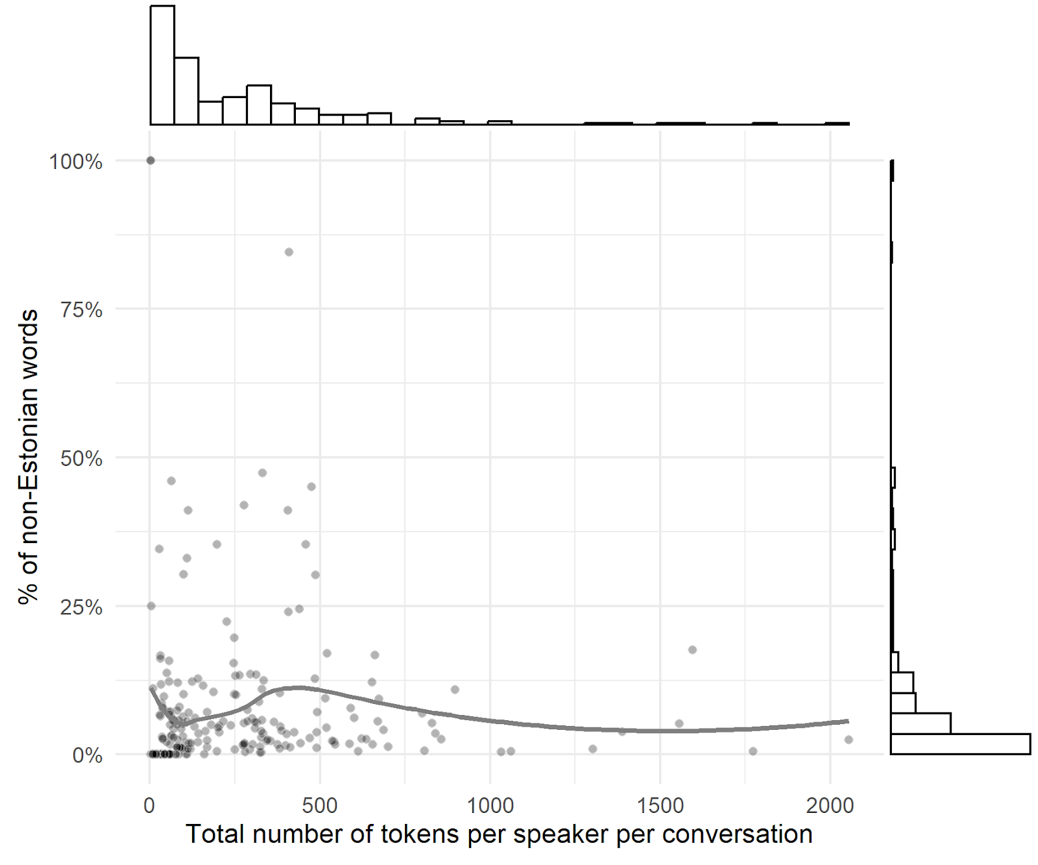
\includegraphics[width=\textwidth]{figures/vihmanetal-img001.png}
\caption{\label{fig:vihmanetal:1}Percentage of non-Estonian tokens, according to the number of total tokens per speaker per conversation in the Estonian Teen Speech IM chat corpus. The histograms on the sides show the overall distribution of the number of tokens (top) and the percentage of non-Estonian words (right) in the conversations per speaker}
\end{figure}


The texts were manually annotated for language choice by a group of researchers and students of linguistics and checked for consistency by the authors. In order to decide whether a “borderline” word is a code-switch or an established loan, we discussed each word, making reference to its inclusion (and labelling as colloquial) in the comprehensive online dictionary,\footnote{\url{https://sonaveeb.ee/} (16 October, 2023). The dictionary has adopted an inclusive approach, including words such as \textit{tšillima}, \textit{tsillima} (from the English ‘to chill’), marked as colloquial. The orthographically unintegrated \textit{chillima,} however, is not included.} its use in other corpora and the coders’ language experience. \citet{VihmanEtAl2022} report that 7.5\% of the words used in the same chat corpus were English (compared to 3.3\% in spoken conversations), but that this fluctuates by speaker and conversation. While this percentage is expected to be lower in longer texts, a great deal of variation exists even in shorter conversations; \figref{fig:vihmanetal:1} shows the length in tokens (including words, emojis and other visual items) for each participant on the x-axis, and the proportion of words in languages other than Estonian on the y-axis.

For the purpose of this study, all tokens marked as non-Estonian, along with their surrounding context, were extracted from the data. Consecutive non-Estonian words were automatically grouped into multiword expressions (compounds, phrases, and sentences). This resulted in an initial dataset with 2269 observations. After manual inspection and correction of the automatic annotations, 2260 observations remained, of which 2234 (98.85\%) were in English, followed by 16 in Russian (0.71\%), 8 in French (0.35\%), and 2 in Finnish (0.09\%). In the final dataset, only the English observations were used.

Out of the 102 participants in the chat corpus, only 3 use Estonian exclusively in their IM conversations. This means that our final dataset contains data from 99 participants, 70\% of whom are female (\figref{fig:vihmanetal:2}).~

  
\begin{figure}
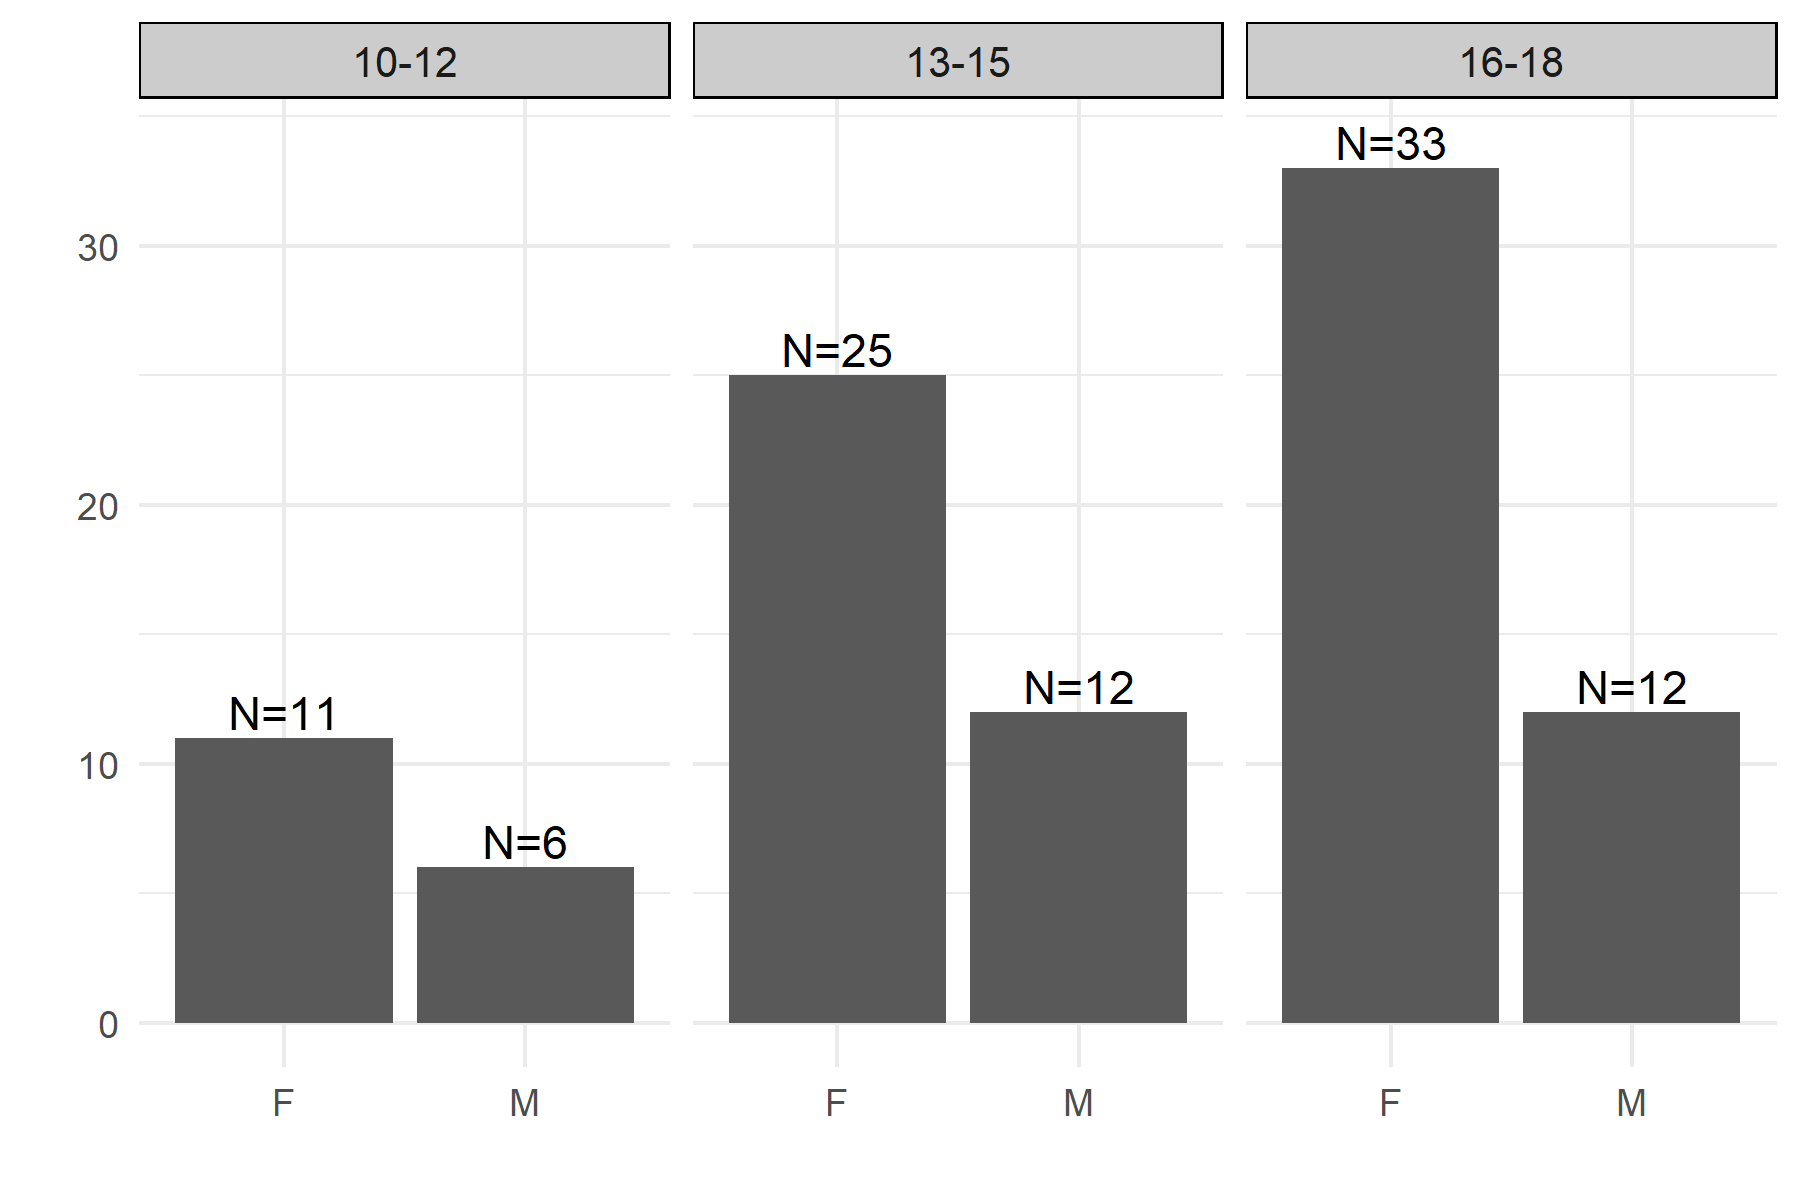
\includegraphics[width=\textwidth]{figures/vihmanetal-img002.png}
\caption{\label{fig:vihmanetal:2} Unique participants (N=99) in the final dataset by gender and age group}
\end{figure}

In all age groups, but especially among the youngest participants, the average rate of English usage is higher for boys (\figref{fig:vihmanetal:3}). However, according to Wilcoxon rank-sum tests, the differences between genders are not statistically significant (all \textit{p-}values exceed .05), although in the youngest group, this results from the presence of outliers and a small sample size.

  
\begin{figure}
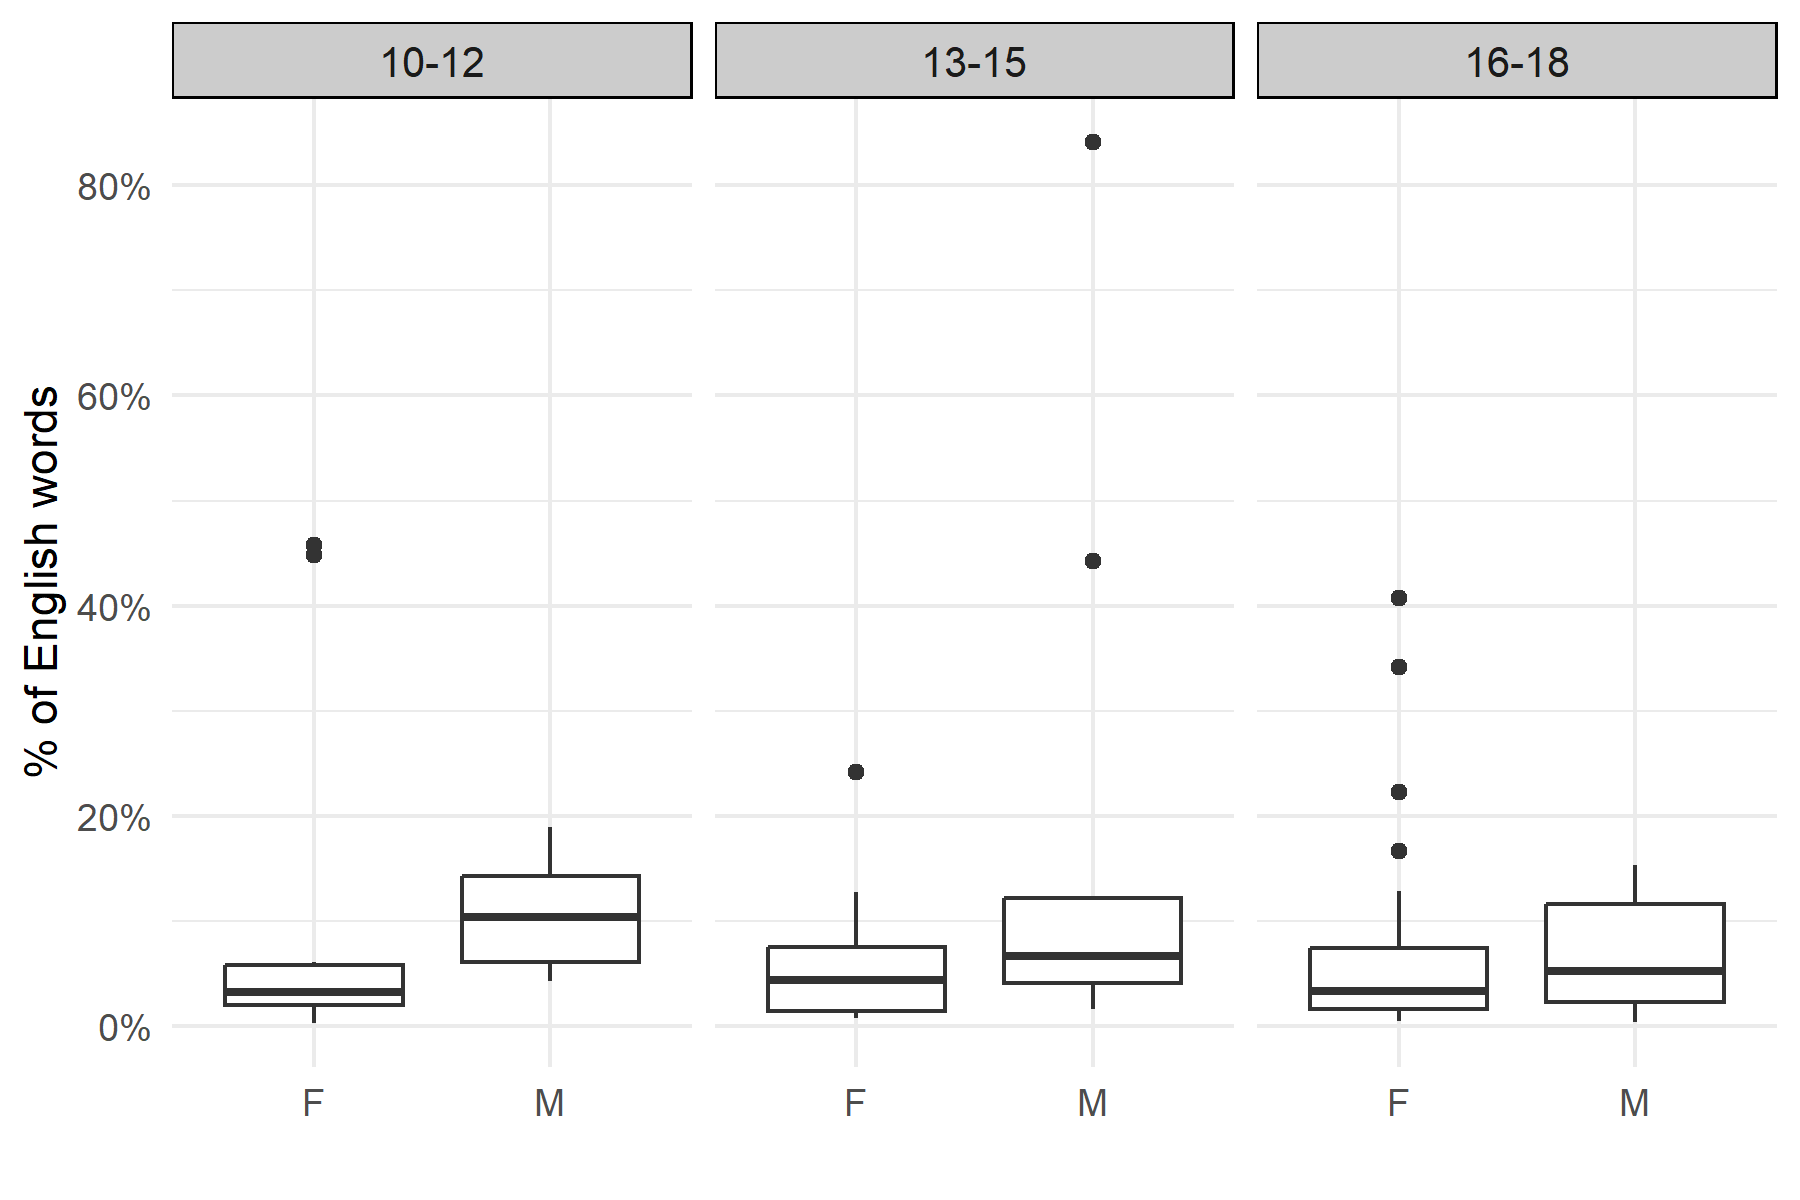
\includegraphics[width=\textwidth]{figures/vihmanetal-img003.png}
\caption{\label{fig:vihmanetal:3} Percentage of English words used by the participants by gender and age group}
\end{figure}

\subsection{Principles for coding code-switching}\label{sec:vihmanetal:3.2}

All observations in the dataset were coded by the authors, in frequent discussion for purposes of reliability and consistency, with regard to their functional category in the turn as well as their orthographic and morphological integration into Estonian. This allowed us to examine which English elements are most often used, and which linguistic expressions are integrated into Estonian. See \tabref{tab:vihmanetal:3} for a summary of the coding system used, along with examples of each category (the dataset and coding principles are also publicly available at \url{https://osf.io/yge27/}).

The coding of a functional category generally coincides with part-of-speech tagging (e.g., conjunctions, interjections, adverbs, nouns, verbs, adjectives), but we also categorized larger units such as fixed phrases and sentences. Although coded separately, in this study, noun phrases, adjective phrases, and verb phrases are subsumed under the corresponding general part-of-speech tags (N, A, and V, respectively) due to their infrequent use. Direct quotes (e.g., from song lyrics) are assigned a separate category.

\begin{table}
\begin{tabularx}{\textwidth}{@{}l@{}lQ}
\lsptoprule
% \textbf{Coding} \textbf{category}
% & \textbf{Level} & \textbf{Examples}\\
\multicolumn{3}{l}{ {Functional category}}\\
\midrule
& adjective & \textit{Pizzatastic}, \textit{coolcoolcool}\\
& adverb & \textit{prolly} ‘probably’, \textit{btw} ‘by the way’\\
& conjunction & \textit{cuz} ‘because’, \textit{tho} ‘though’ \\
& noun & \textit{playlist}, \textit{DUMBASS}\\
& verb & \textit{join-i-da} ‘to join’, \textit{SPOIL-I-MA} ‘to spoil’\\
& interjection & \textit{brooo}, \textit{Jeaa} ‘yeah’\\
& question word & \textit{howwwww}, \textit{wut} ‘what’\\
& phrase & \textit{I guess}, \textit{oh well}\\
& quote & \textit{Thank you next}, \textit{I got tha moves like jagger}\\
& sentence & \textit{and where u at}, \textit{less goo} ‘let’s go’\\
\tablevspace
\multicolumn{3}{l}{\textbf{Orthographic integration}}\\
\midrule
& yes & \textit{oomaigad} ‘oh my god’, \textit{kamooon} ‘come on’, \textit{oukei} ‘okay’\\
& no & \textit{Alrightt}, \textit{yeeee}, \textit{GREEN SCREEN-I-GA} ‘with a green screen’\\
& mixed & \textit{scämm} ‘scam’, \textit{cropp top-i-d} ‘crop tops’, \textit{hope iz uki} ‘hope (it) is okay’\\
& NA & \textit{Ikr} ‘I know right’, \textit{WDYM} ‘what do you mean’, \textit{Lvl up} ‘level up’\\
\tablevspace
\multicolumn{3}{l}{\textbf{Morphological integration}}\\
\midrule
& yes & \textit{ma tulen} \textbf{\textit{gym-i-st}} ‘I’m coming from the gym’, \textit{Nii hea} \textbf{\textit{edit-i-ja}} ‘such a good editor’, \textit{mulle ei meeldi} \textbf{\textit{reality-t}} \textbf{\textit{face-da}} ‘I don’t like to face reality’\\
& no & \textit{tahaks teha seda} \textbf{\textit{challenge} }(: \textit{challenge’i}) värki ‘I’d want to do that challenge thing’, \textit{hessi friikad on} \textbf{\textit{soggy}} (: \textit{soggy’d}) ‘Hesburger’s fries are soggy’, \textit{mingid} \textbf{\textit{fancy}} (: \textit{fancy’d}) \textit{veinipokaalid} ‘some fancy wine glasses’\\
& NA & \textbf{\textit{i} \textbf{\textit{need}} \textbf{\textit{to}} \textbf{\textit{go}} }\textit{niitma} ‘I need to go mow the lawn’, \textit{ma} \textbf{\textit{probably} }\textit{votan need} ‘I’ll probably take these’, \textit{okei see on} \textbf{\textit{ylinaiss} }‘okay that’s really nice’\\
\lspbottomrule
\end{tabularx}%%please move \begin{table} just above \begin{tabular
\caption{Summary of coding categories with examples. If an example contains an Estonian word with nonstandard spelling, the standard orthographic form will be presented in square brackets [: ]; if the example contains an Estonian word with nonstandard morphology, the standard form will be presented in round brackets (: ).}
\label{tab:vihmanetal:3}
\end{table}


\clearpage
We considered the inserted elements to be orthographically integrated when their spelling deviates from their expected (standard or nonstandard, e.g., \textit{bruh} as used in English-context IM language) spelling in the source language, which in this case is English. This happens when the speakers integrate English into the phonetically transparent Estonian orthography (\textit{is veri guud} < ‘is very good’, \textit{dunt vörri} < ‘don’t worry’, \textit{verinaiss} < ‘very nice’). In some cases, especially with compounds, phrases, and sentences, but also with some simplex words, only part of the expression is integrated (\textit{thankjuu} < ‘thank you’, \textit{whateefak} < ‘what the fuck’), in which case the items were coded as exhibiting mixed orthographic integration. Abbreviations, such as \textit{wym} ‘what [do] you mean’ and \textit{omg} ‘oh my god’, were considered difficult to assess for (non-)integration, and they were marked as NA (not applicable).

Non-Estonian words and expressions in the chats were coded for being morphologically integrated when they incorporated elements from Estonian inflectional (and, occasionally, derivational) morphology. This mainly concerns nouns (\textit{bag-i-d} bag{}-\textsc{tv-pl} ‘bags’), adjectives (\textit{clean-i-m} clean{}-\textsc{tv-cmp} ‘cleaner’), and the corresponding phrases, which allow for inflectional marking for case, number, and degree, as well as verbs (\textit{quitt-i-sin} quit{}-\textsc{tv}{}-1\textsc{sg.pst} ‘(I) quit’) and verb phrases (\textit{reality-t face-da} reality{}-\textsc{sg.par} face{}-\textsc{inf} ‘to face reality’). The items were coded with NA when the grammatical function did not require any use of inflectional morphology in Estonian (e.g., the unmarked nominative singular case, imperative mood for some inflectional verb types, other parts of speech, such as adverbs, interjections, conjunctions, and fixed phrases and sentences). English elements were coded as not being morphologically integrated when their grammatical function would call for such marking in standard Estonian, but the speakers had either left them unmarked or used the morphology from the source language. Therefore, the binary opposition between morphologically marked and unmarked elements in our data only reflects whether the potential for morphological integration in specific contexts was realized or not.


\section{Results}\label{sec:vihmanetal:4}
\subsection{English code-switches by category}\label{sec:vihmanetal:4.1}

In this study, since we are interested in the integration of words and phrases both orthographically and morphologically into Estonian-language contexts, we are especially interested in intrasentential usage. Hence, we first report the proportions with which English-language segments of all kinds (including full turns and whole sentences) are used in the data and then limit our focus to sub-utterance level switched elements.\footnote{All linguistic examples are presented in their original typographical form.} We also exclude titles and quotes (especially song lyrics) from further analysis, to the extent that we were able to identify them.

  \begin{figure}[t]
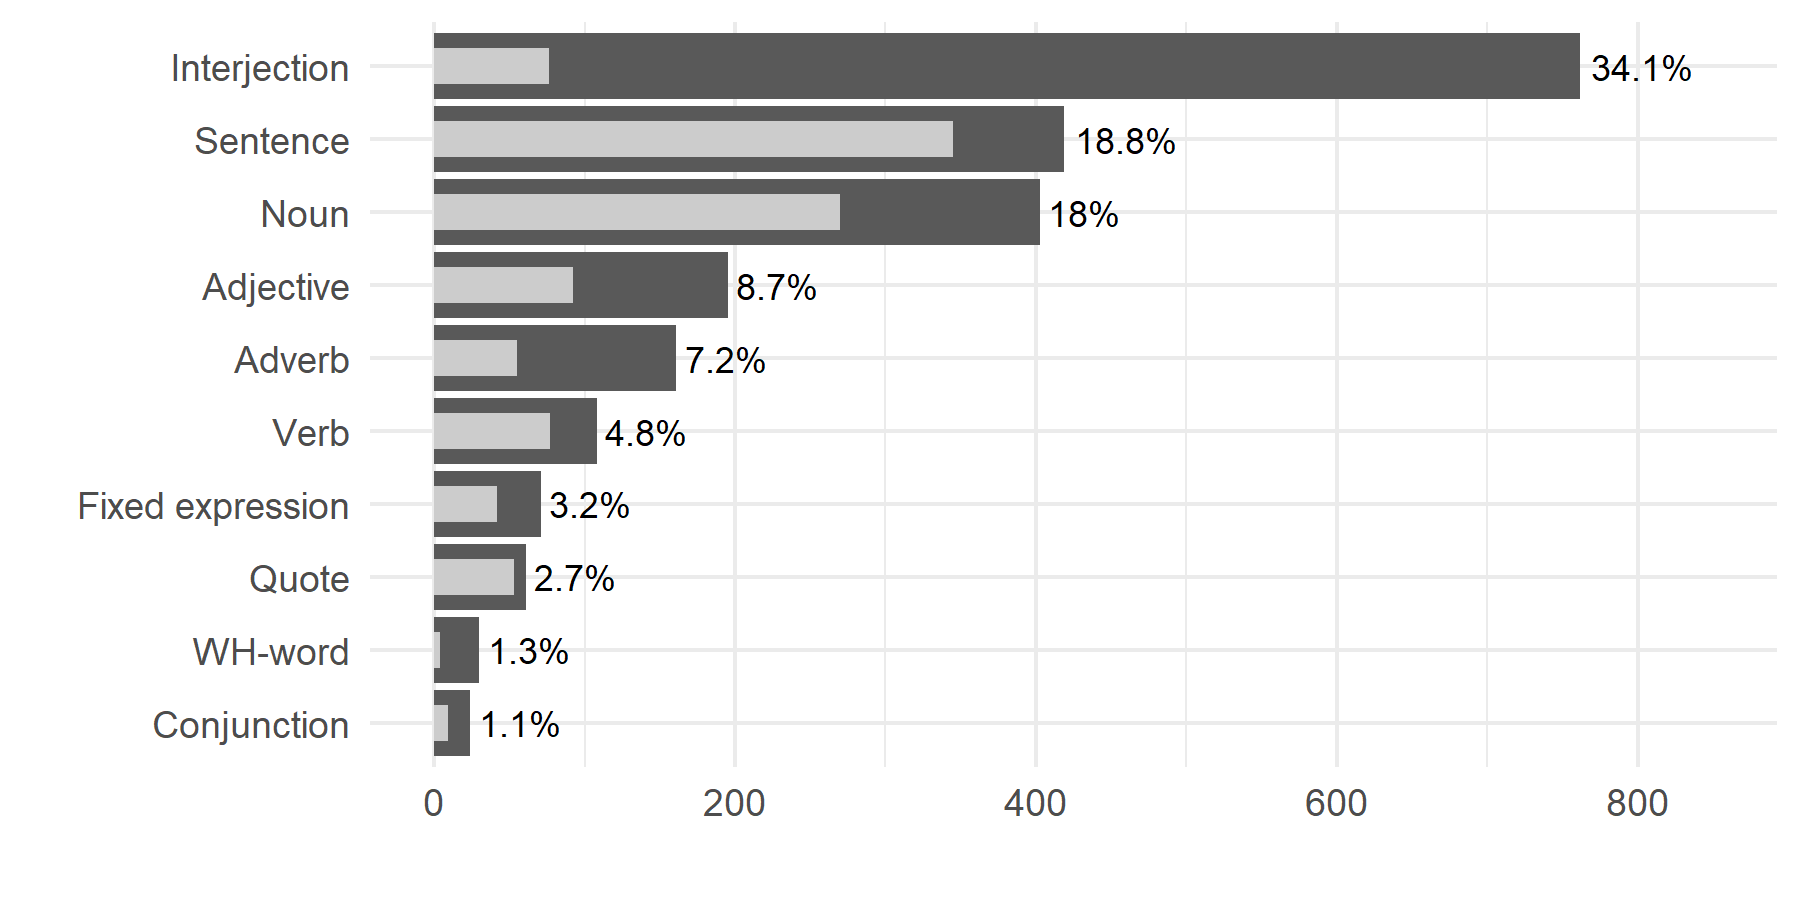
\includegraphics[width=\textwidth]{figures/vihmanetal-img004.png}
  \caption{\label{fig:vihmanetal:4} The categorical distribution of English expressions by tokens (dark grey bars) and standardized types (light grey bars)}
\end{figure}

As can be seen in \figref{fig:vihmanetal:4}, 53\% (N=1181) of the English expressions in our dataset occur in intersentential positions, where the segments are not syntactically linked to the preceding or succeeding context. These exclude quotes (which have both inter- and intrasentential uses) and include simplex and multiword interjections (e.g., ‘wow’, ‘oh my god’) and sentences. However, the numbers of unique standardized types (e.g., ‘please’) corresponding to the various surface forms of the interjections (e.g., \textit{please}, \textit{pliis}, \textit{pliizzzz}) show that the participants make repeated use of a relatively small set of expressions in the interjection category. This also holds for adjectives and adverbs, where unique types make up less than half of all attested tokens. The most common types and their realizations are discussed in the following subsections.

\subsection{Orthographic integration} \label{sec:vihmanetal:4.2}

Overall, non-integration into Estonian orthography is more common than Estonianized spelling. Nearly one-fifth (17.2\%, N=374) of English elements were coded as NA for orthographic integration, meaning that integration was not an option; these mostly include abbreviations (e.g., \textit{btw} ‘by the way’, \textit{lmao} ‘laughing my ass off’, \textit{lol} ‘laugh out loud’, \textit{wtf} ‘what the fuck’, \textit{fr} ‘for real’). Out of the codable tokens, 83\% (N=1492) were unintegrated orthographically, 13.7\% (N=247) were integrated, and 3.3\% (N=60) were coded as mixed. Mixed integration indicates that elements of English spelling and Estonian-based spelling were used. English spelling includes letters used only in loanwords in Estonian (e.g., Q in ‘quit’, C in ‘creepy’, Y in ‘yo’, ‘actually’), as well as the many orthographic representations in English which do not map phonemes to letters. Estonianized, or integrated, spelling in mixed words is seen, among other features discussed below, in spelled-out diphthongs (e.g., \textit{noupp} < ‘nope’), the use of Estonian diacritics (\textit{scämm} < ‘scam’, or \textit{dunt vörri} < ‘don’t worry’), and Estonian vowels used in place of English spelling (\textit{in realati} < ‘in reality’). When a speaker corrected themselves, we did not count the nonstandard spelling. Otherwise, we cannot rule out the possibility that some nonstandard spelling arises from misspelled words or unintentional typos, but the extent and systematic nature of the Estonianized spellings indicates that this is a commonly used device.

Not all speakers make equal use of the option to integrate the English elements into Estonian orthography. Among the 86 speakers (out of 99) who contributed at least 4 codable (i.e. non-NA) observations to the dataset, the integration rates ranged from 0 to 100 (\textit{M}=25.2\%, \textit{SD}=25.5\%, \textit{Mdn}=17\%). Interestingly, the youngest age group (ages 10--12) made considerably less use of orthographic integration than the older age groups (\textit{M}=13.5\%, \textit{SD}=12.4\%, \textit{Mdn}=8.3\%). However, the integration rates are also influenced by the functions in which the English elements are used. 

As \figref{fig:vihmanetal:5} shows, interjections are not only the most frequent English-language elements but also the most frequently integrated orthographically. In this section, we examine interjections, with their high rate of 28.3\% integrated (N=216, including mixed) spellings, verbs (18.5\%, N=20), adjectives (13.8\%, N=27), and nouns (6.5\%, N=26). If we consider only codable items (excluding NAs), the integration rates of interjections, verbs, adjectives, and nouns are 41\%, 18.5\%, 14\%, and 7\%, respectively. A table for the data in \figref{fig:vihmanetal:5} is given in the Appendix (Table \ref{tab:vihmanetal:a1}).

  
\begin{figure}[p]
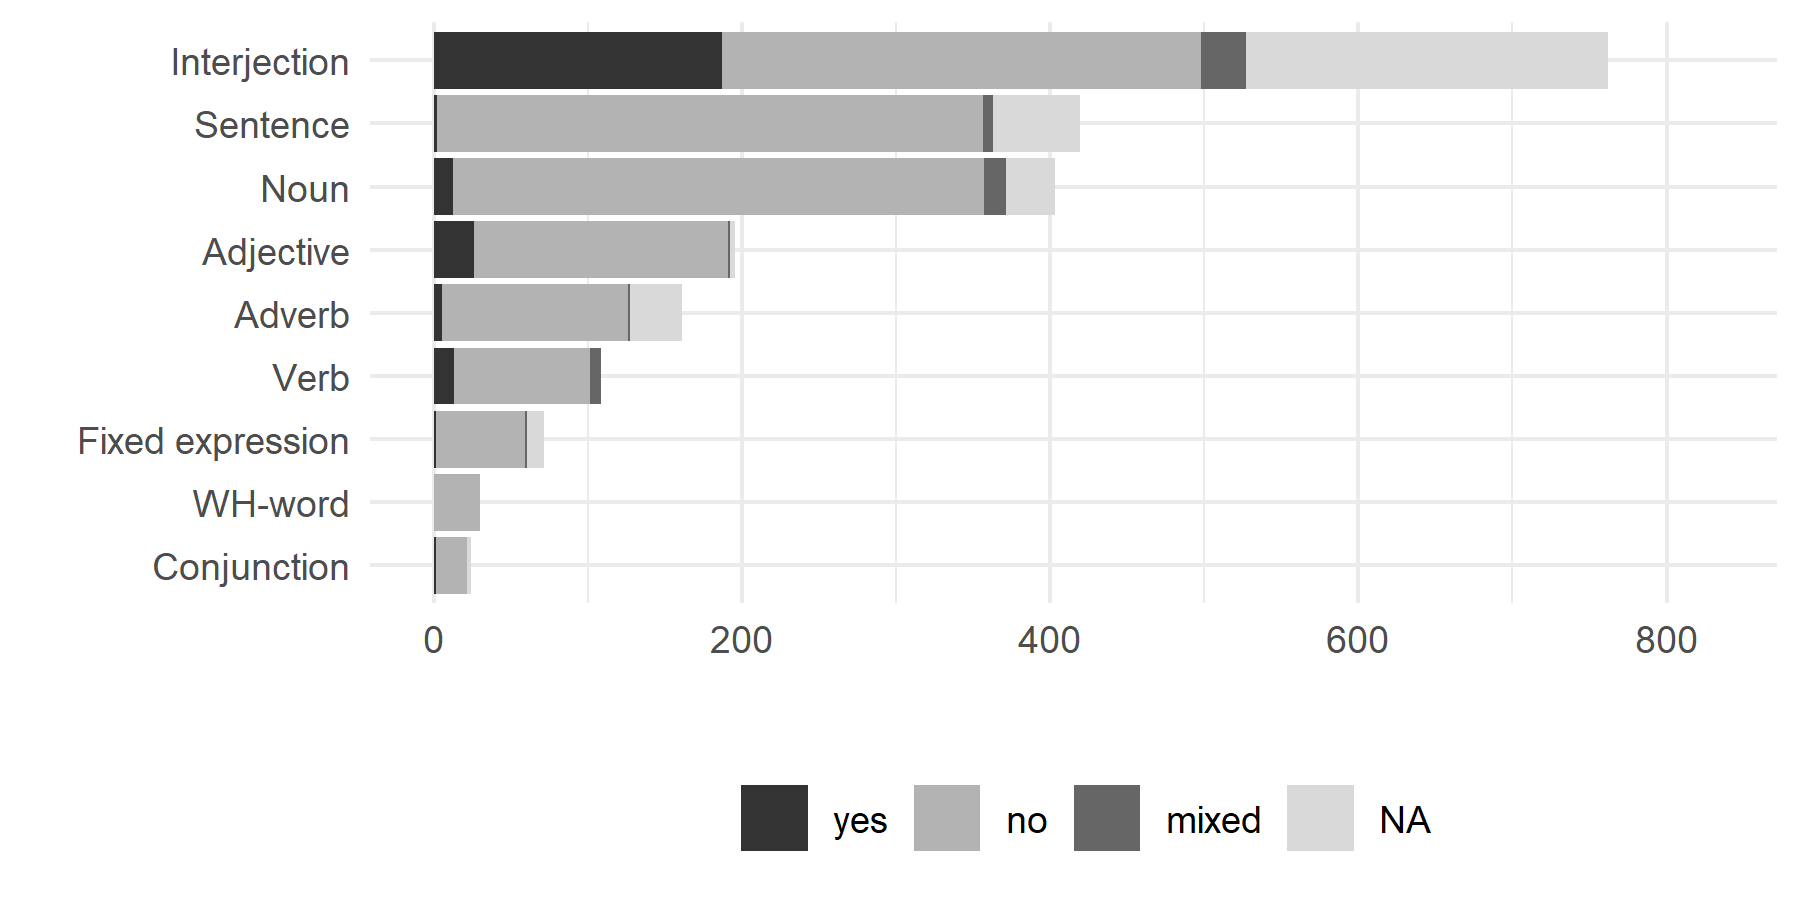
\includegraphics[width=\textwidth]{figures/vihmanetal-img005.png}
\caption{\label{fig:vihmanetal:5} Orthographic integration by category (yes = orthographically integrated, no = unintegrated)}
\end{figure}

\subsubsection{Interjections}\label{sec:vihmanetal:4.2.1}

\begin{table}[p]
\small
  \caption{Orthographic integration of the most frequently used English-language interjections}
  \fittable{
\begin{tabular}{p{1.7cm}@{}r>{\raggedleft}p{1.5cm}p{3.5cm}p{3.9cm}}
\lsptoprule
 {Standard}  {expression} &  {N}  {tokens} &  {N}  {spelling}  {variants} &  {Examples:}  {orthographi\-cally}  {integrated,}  {mixed}  &  {Examples:}  {not}  {orthographi\-cally}  {integrated}  {or}  {NA}\\
\midrule
‘laughing out loud’ & 115 & 3 & {}- & \textit{lol, lolol, looooooooool}\\
\tablevspace
‘yup’ & 65 & 15 & \textit{jep, jap, jaaap} & \textit{yep, yepp, yup}\\
\tablevspace
‘yo’ & 53 & 16 & \textit{jo, jou, joou, joukijou, you, yoooooou} & \textit{yo, yoooo, yoyo}\\
\tablevspace
‘yes’ & 49 & 23 & \textit{jaas, jes, jesss} & \textit{yes, yas, yaaass, yesh, yasshshhhhh}\\
\tablevspace
‘yay’ & 39 & 13 & \textit{jee, jeii, jeje, jeiii, yeyy} & \textit{yay, yayyyyyyyyyyyyyyyyyyy}\\
\tablevspace
‘please’ & 34 & 15 & \textit{pliiiiiiiiiiiiiiiiiiiiiiiiiiiiiissss} & \textit{please, pls, plsss, plz, plzzzz}\\
\tablevspace
‘yeah’ & 33 & 19 & \textit{je, jee, jea, jeeeaaa, jeah} & \textit{ye, yea, yeah, yeye}\\
\tablevspace
‘sorry’ & 32 & 9 & \textit{sori, sorri} & \textit{sorry, sorryy, sry, srryyyy, sryyy}\\
\tablevspace
‘aww’ & 28 & 14 & \textit{awii, awsii} & \textit{aw, awh, aww}\\
\tablevspace
‘wow’ & 27 & 5 & \textit{vauu, vov} & \textit{wow, woow, wowowo}\\
\lspbottomrule
\end{tabular}
}
\label{tab:vihmanetal:4}
\end{table}


Most of the orthographic integration occurs in frequently used interjections (41\% of codable items). The most frequent English-language interjections are shown in \tabref{tab:vihmanetal:4}. These include abbreviations characteristic of IM language internationally (\textit{lol} ‘laugh[ing] out loud’, \textit{omg} ‘oh my god’), and commonly used words in English (‘yeah’, ‘wow’, ‘sorry’). They range from three orthographic variants of ‘lol’ to 23 variants of ‘yes’, 19 variants of ‘yeah’, and 15 of ‘yup’ (the last three could also be grouped together as the affirmative particle). While most of the variation can be classified under features typical of internet language – pronunciation-based spelling, lengthening words by repeated letters or syllables, and shortening words by letter omission – we also find examples in the more frequent interjections of both integrated and non-integrated spelling variants, both within and across speakers.


Some further frequent interjections with varying forms include ‘thanks’ (20 tokens/ 9 spelling variants, e.g., \textit{thanks}, \textit{tanks}, \textit{thx}, \textit{tnx}, \textit{tänks}, \textit{tänx}) and ‘thank you’ (11/8, e.g., \textit{thank you}, \textit{tankjuu}, \textit{thankjuuu}, \textit{thankyouuu}, \textit{ty}, \textit{tänkju}), ‘oh my god’ (25/9, e.g., \textit{oomaigad}, \textit{omaikad}, \textit{omg}, \textit{omgk}, \textit{ommmmmgggggggggggggg}), ‘bye’ (12/7, e.g., \textit{bye}, \textit{byeee}, \textit{baiiii}), ‘okay’ (14/9, e.g., \textit{okay}, \textit{ok}, \textit{ouk}, \textit{oukei}, \textit{ooook}, \textit{kkkk}, \textit{okeoke}), and ‘nope’ (13/5, e.g., \textit{nope}, \textit{noupp}, \textit{noouupp}). Note that in expressions like ‘thanks’ and ‘oh my god’, the orthographic rendition tends to be internally consistent: the Estonian -\textit{ä}{}- does not co-occur in our corpus with the English word-initial \textit{th}{}-; similarly, the spelling \textit{mai} for ‘my’ appears with \textit{gad}, but never with the English spelling \textit{god.} On the other hand, with such rampant variability, this is clearly not a hard constraint: we also find mixed orthography such as \textit{jeah} ‘yeah’ and \textit{thankjuuu} ‘thank you’.

The spelling variants of both orthographically integrated and non-integrated forms are, of course, not equally distributed and some variants are clearly more conventionalized both in terms of their overall usage frequency as well as their spread across different speakers. For example, out of the 65 uses of ‘yup’, 24 occur in the form of \textit{jep} and 22 in the form of \textit{jap}. \textit{Jep}, in turn, is used by 15 different speakers, while \textit{jap} is used by 10 different speakers. The other spelling variants occur 1-2 times and are also used by 1-2 speakers. However, our corpus is currently too small to make a sufficiently credible distinction between individual innovations and spellings more widely accepted in the community, especially for the expressions whose overall frequency in the corpus is lower.

\subsubsection{Verbs}

While only 108 tokens of English verbs and verb phrases were found in our corpus, 18.5\% of these were coded as orthographically either integrated or mixed. The English verbs are frequently given a geminated stem-final consonant before Estonian inflectional morphology (e.g., \textit{cropp-i-nd} crop{}-\textsc{tv-app} ‘cropped’\textit{, tripp-i-da} trip{}-\textsc{tv-inf} ‘to trip’\textit{, lagg-a-b} lag{}-\textsc{tv-3sg.prs} ‘lags’\textit{, robb-i-b} rob{}-\textsc{tv-3sg.prs} ‘robs’\textit{, quitt-i-sin} quit{}-\textsc{tv-1sg.pst} ‘(I) quit’\textit{, snäpp-i-sid} snap-\textsc{tv-2sg.prs} ‘(you) snapped’). From these same examples, we can see some lexical variation in theme vowel selection, with both the default -\textit{i} and -\textit{a} used.

Some other modifications are also connected to the way stems behave before inflectional endings, such as the omitted W at the end of ‘follow’ in example \REF{ex:vihmanetal:1a} and the partially integrated ‘invite’ in (1b-c). Examples (1b-c), from boys of similar ages, show variation: \REF{ex:vihmanetal:1b} uses a short form of the verb stem (\textit{inva}), more adapted to Estonian morphophonology, possibly indicating loanword status, while \REF{ex:vihmanetal:1c} uses the full English stem ‘invite’, but adopts Estonian consonant gradation, according to which the /t/ occurs in its weak form and is written with -\textit{d}. This orthography shows adaptation to Estonian, yet the diphthong /aɪ/ is left unintegrated, with English spelling.

\ea%1
    \label{ex:vihmanetal:1}
\ea   (M, 12)\\ \label{ex:vihmanetal:1a}
\gll {Yks [: Üks]} kuulsus \textbf{{follo-b}} min-d\\
one    celebrity  \textbf{follow{}-3}\textbf{\textsc{sg.prs}}  1\textsc{sg.par}\\
\glt  ‘A celebrity is following me.’

\ex  (M, 13)\\ \label{ex:vihmanetal:1b}
\gll Mä   käsi-n     sin-d     \textbf{{inva-da}}\\
1\textsc{sg}  order-1\textsc{sg.prs}  2\textsc{sg.par}  \textbf{invite-\textsc{inf}}\\
\glt ‘I command [them] to invite you.’

\ex  (M, 11)\\ \label{ex:vihmanetal:1c}
\gll probleem  on    selle-s    et  sa \textbf{{invid-i-d}}    min-d    mängi-ma,  mitte vaata-ma\\
problem  be.3\textsc{sg.prs}   this-\textsc{sg.ine}   that  2\textsc{sg} \textbf{invite-\textsc{tv-2sg.prs}}   1\textsc{sg.par}   play-\textsc{inf}   \textsc{neg} watch-\textsc{inf}\\
\glt ‘The problem is that you’re inviting me to play not to watch.’
\z
\z



\subsubsection{Adjectives}

Adjectives follow interjections and verbs in terms of proportion of orthographic integration (14\% of codable items are integrated). The most frequently attested English adjectives are listed in \tabref{tab:vihmanetal:5}, along with examples of integrated and non-integrated variants. ‘Nice’ is used much more than any other adjective, with tokens nearly evenly divided between integrated Estonian spellings (varying between one and four S’s) and unintegrated variants. ‘Nice’ (pronunciation spelling > \textit{naiss}) is also used in compounded adjectives with Estonian intensifying modifiers meaning ‘very’ and ‘super’ (\textit{väganaiss} ‘very nice’, \textit{ylinaiss} ‘super-nice’) and English ones (\textit{verinaiss} ‘very nice’). Three examples are attested in the corpus of compound adjectives formed with a prefixal form of ‘very’, two of which have integrated spelling\footnote{Note that the Estonianized \textit{veri} for ‘very’ is isomorphic with \textit{veri} ‘blood’.} (\textit{verinaiss} and \textit{verikhuul} ‘very cool’), and one retains English spelling (\textit{verygood}); note that both examples with \textit{veri} also have Estonianized orthography for the adjective itself, whereas \textit{verygood} retains English orthography for both compound elements.

The adjectives ‘fine’ and ‘cool’ are attested with both integrated and unintegrated variants. Interestingly, integrated ‘cool’ (\textit{khuul}) is spelled in such a way as to indicate orthographic \textit{but not phonological} integration: the H represents anglicized aspiration, a phonological feature that stands out in Estonian, which has unaspirated stops.

Finally, ‘true’, ‘cringe’, ‘fucked up’, ‘hot’, ‘sad’, and ‘ugly’ are not attested with integrated variants. Even though ‘true’, ‘ugly’, and ‘cringe’ also occur in nonstandard English spelling, these deviations are not aligned with Estonian orthography.

\begin{table}[t]
  \caption{Orthographic integration of the most frequently used English-language adjectives}
\begin{tabularx}{\textwidth}{QrYQQ}
\lsptoprule
{Standard} {expression} & {N} {tokens} & {N} {spelling} {variants} & {Examples:} {integrated,} {mixed}  & {Examples:} {not} {integrated} {or} {NA}\\
\midrule
‘nice’ & 41 & 12 & \textit{nais, naissss, naissu} & \textit{nice, noic, niceee}\\
‘fine’ & 7 & 3 & \textit{fain} & \textit{fine}\\
‘true’ & 7 & 4 & {}- & \textit{true, tru, truuuue} \\
‘cool’ & 6 & 4 & \textit{khuul} & \textit{cool, coolcoolcool}\\
‘cringe’ & 5 & 2 & {}- & \textit{cring, cringe}\\
‘fucked up’ & 5 & 1 & {}- & \textit{fucked up}\\
‘hot’ & 5 & 2 & {}- & \textit{hot}\\
‘sad’ & 5 & 1 & {}- & \textit{sad}\\
‘ugly’ & 5 & 2 & {}- & \textit{ugle, uglee}\\
\lspbottomrule
\end{tabularx}%%please move \begin{table} just above \begin{tabular
\label{tab:vihmanetal:5}
\end{table}

Interestingly, the most frequently used English adjectives can often be found in similar contexts as interjections, i.e., in intersentential positions where they function as complete turns expressing immediate reactions to the interlocutor’s message. This becomes especially relevant when considering their low availability for morphological integration (see \sectref{sec:vihmanetal:4.3}).

\subsubsection{Nouns}

More English nouns are used than verbs, but a smaller proportion of the nouns are orthographically integrated. Out of 371 codable (integratable) nouns, only 7\% are coded as integrated or mixed. Most of these are unique items. The only orthographically integrated nouns occurring with a frequency greater than one are \textit{spammi} ‘spam’ and \textit{vaib} ‘vibe’. ‘Spam’ occurs once with English orthography and twice with two M’s, as shown in example \REF{ex:vihmanetal:2}. In both cases, the double letter m seems to be driven by the case inflection -\textit{i}, which marks this word as either partitive \REF{ex:vihmanetal:2a} or genitive \REF{ex:vihmanetal:2b}. The word-medial vowel is left unintegrated, but in both examples, the texter has also left diacritics off of Estonian words (\textit{akki} pro ‘äkki’ in 2a; \textit{parast} pro ‘pärast’ in 2b), and hence this can be interpreted as their rapid messaging style.

\ea%2
    \label{ex:vihmanetal:2}
\ea   (M, 12)\\ \label{ex:vihmanetal:2a}
\gll  {Akki [: Äkki]}  ta   ei  taht-nud \textbf{{spamm-i} }{[: spämmi]}\\
maybe    \textsc{3sg}  \textsc{neg}  want-\textsc{app}  \textbf{spam-\textsc{sg.par}}\\
\glt  ‘Maybe s/he didn’t want spam.’

\ex(F, 10)\\ \label{ex:vihmanetal:2b}
\gll  (sry   {\textbf{spamm-i} [: spämmi]}  {parast [: pärast]}  XD)\\
sorry   \textbf{spam-\textsc{sg.gen}}    because-of    XD\\
\glt ‘Sorry because of the spam [XD= laughing emoticon].’
\z
\z




Nouns and verbs are examined more closely in \sectref{sec:vihmanetal:4.3}.

\subsection{Morphological integration}\label{sec:vihmanetal:4.3}

Morphological integration is not directly comparable to orthographic integration. First, morphology is not available in all contexts in the way orthographic choices usually are. Whereas over 80\% of English items were marked as codable for orthography, the converse is the case for morphological integration: only 13.5\% (N=294) were marked as codable. Therefore, the vast majority (86.5\%, N=1879) represent elements which are unintegrated grammatically. These include interjections (described above), independent and tag phrases (e.g., \textit{all good}, \textit{fingers crossed}, \textit{no pressure}, \textit{i guess}) and sentences (e.g., \textit{and you gave yourself a unfair advantage}, \textit{i ate cheeseballs}, \textit{im giving tough love}, \textit{it do be like that}, \textit{then we can eat butt load of pasta}), as well as words which can be seen as integrated grammatically without any additional morphology. For instance, adverbs (e.g., \textit{literally}, \textit{prolly} ‘probably’, \textit{offically} ‘officially’, \textit{kinda} ‘kind of’\textit{;} see 3a) are grammatically appropriate without added morphology. Others that need no additional marking are conjunctions \REF{ex:vihmanetal:3b}, nouns, noun phrases and adjectives in nominative singular, which uses bare forms in Estonian and does not have form restrictions \REF{ex:vihmanetal:3c}, and verbs ending with a vowel when they appear in imperative singular, which uses the suffixless verb stem \REF{ex:vihmanetal:3d}.

\ea%3
    \label{ex:vihmanetal:3}
\ea  (F, 13)\\ \label{ex:vihmanetal:3a}
\gll Ta  \textbf{{offically}}  vihka-b     min-d\\
3\textsc{sg}  \textbf{officially}  hate{}-3\textsc{sg.prs}  \textsc{1sg-par}\\
\glt ‘S/he officially hates me.’

\ex  (F, 17)\\ \label{ex:vihmanetal:3b}
\gll ja   markkus  sa-i     täiega  vihase-ks   \textbf{therefore}   me   pol-nud   terve     päeva     rääki-nud\\
and   Markkus get{}-\textsc{3sg.pst}   totally   mad{}-\textsc{sg.tr}   \textbf{therefore}   \textsc{1pl}  \textsc{neg.aux-app}   whole.\textsc{sg.gen}  day.\textsc{sg.gen}   talk{}-\textsc{app}\\
\glt ‘And Markkus got really angry, therefore we hadn’t spoken the whole day.’

\ex  (F, 12)\\ \label{ex:vihmanetal:3c}
\gll Sa   ole-d     mu     \textbf{best} \textbf{friend}\\
2\textsc{sg}  be{}-3\textsc{sg.prs}   \textsc{1sg.gen}   \textbf{best} \textbf{friend}\\
\glt ‘You’re my best friend.’

\ex   (M, 11)\\ \label{ex:vihmanetal:3d}
\gll Lihtsalt     \textbf{{copy}}     lingi\\
simply     \textbf{copy.\textsc{2sg.imp} }  link.\textsc{sg.gen}\\
\glt ‘Just copy the link.’
    \z
\z


Turning to the smaller proportion of items determined to be codable for morphological integration (N=294), the results are again complementary to those for orthographic integration: 79\% (N=232) are morphologically integrated, and only 21\% (N=62) lack relevant morphology.

The rates of morphological integration also vary less between different speakers than those of orthographic integration. Since there are considerably fewer codable items, there are only 24 speakers (out of 99) who contributed at least 4 codable observations to the dataset. Among them, integration rates range from 50\% to 100\% (\textit{M}=83.5\%, \textit{SD}=15.3\%, \textit{Mdn}=79.6\%) and there seem to be no significant differences between the different age groups.

\figref{fig:vihmanetal:6} shows the proportions of morphologically integrated English-lan\-guage elements by category. If we leave aside the code-switched elements marked as NA, we find that both nouns and verbs show equally high levels of integration: 81.4\% (N=149) of integratable nouns and 81.2\% (N=69) of integratable verbs are morphologically integrated (37\% of nouns overall compared to 64\% of verbs overall bear Estonian morphological marking, if we also consider NAs); following these are adjectives, which are more or less equally likely to be integrated (53.8\%, N=14) or unintegrated. We look at each of these categories in turn. A table for this data is given in the Appendix (Table \ref{tab:vihmanetal:a2}).

  
\begin{figure}[t]
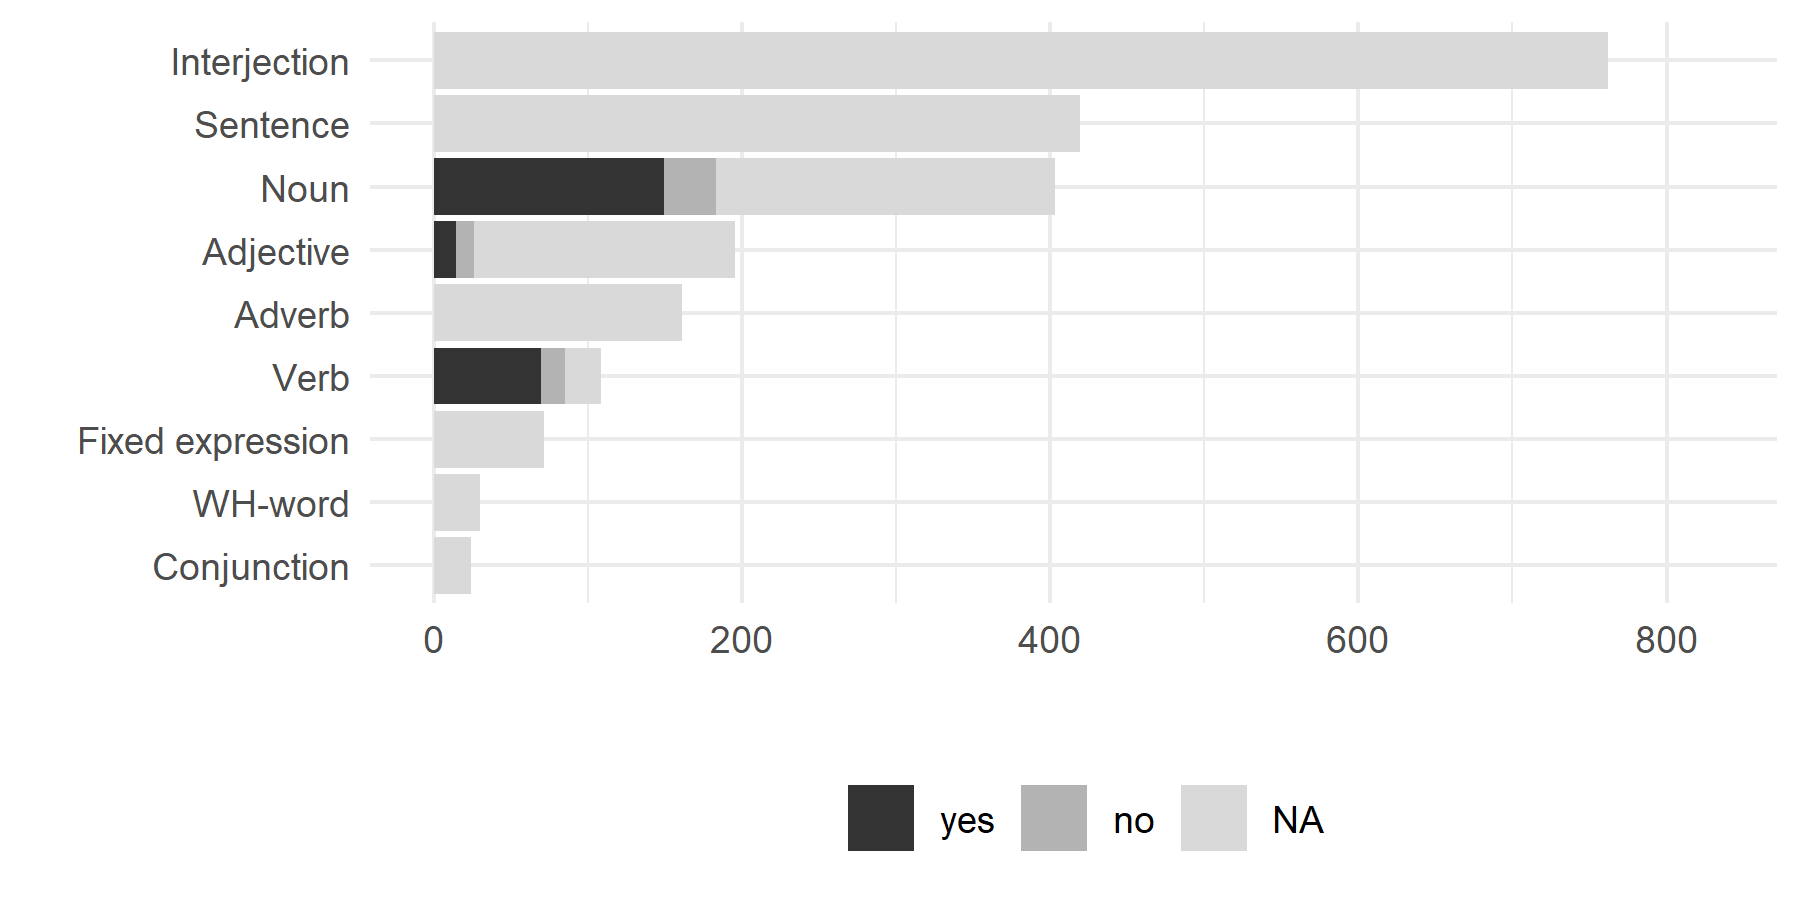
\includegraphics[width=\textwidth]{figures/vihmanetal-img006.png}

\caption{\label{fig:vihmanetal:6} Morphological integration by category}

\end{figure}

\subsubsection{Nouns}

Nouns are reported to be the part of speech most likely to be used in code-switching \href{https://www.zotero.org/google-docs/?ozak2Z}{(\citealt{ThomasonKaufman1988, Field2002})}. The most probable reasons for this are the diversity of referents and the greater likelihood of semantically (and also culturally) specific words used to refer to them \href{https://www.zotero.org/google-docs/?pgMSUx}{(\citealt{BackusVerschik2012})}. In English, it has been suggested that another factor facilitating code-switching is the greater ease of grammatical integration, but in Estonian, this factor cannot play a role, as nominal morphology is complex and frequently required in Estonian clauses. 

Nominative singular nouns (e.g., subjects) do not require any morphological marking, but nearly half (183) of the 403 English nouns and noun phrases in our data are coded as potentially carrying marking, i.e. are codable for morphological integration. Out of these, only 34 (18.6\%) are left unmarked. Many of the unmarked nouns may be treated by the speakers like proper names when they are used in highly semantically specific ways to indicate a button or function in an app or game (\textit{dislike}, \textit{autotune}, \textit{mute}), or other internet-related specific terminology (\textit{fyp} ‘For You page’, \textit{girl defined reaction video, invite to watch}, \textit{lobby}, \textit{Groovepad}; see example 4a). Nevertheless, proper names are also inflected in Estonian. Six nouns and one NP have English plural marking instead of integration (\textit{flames}, \textit{files}, \textit{vibes}, \textit{bikers}, \textit{hips}, \textit{leggings}, \textit{religious school tingz} ‘things’). Example \REF{ex:vihmanetal:4b} shows one of the few examples of an English word (denoting the name of a cafe) clearly requiring a locative ending in Estonian (illative, indicating directionality), which remains unmarked. In most such instances, the English noun is given an Estonian affix, as below in \REF{ex:vihmanetal:5}.

\ea%4
    \label{ex:vihmanetal:4}
\ea (M, 11)\\ \label{ex:vihmanetal:4a}
\gll tea-d      \textbf{{join-i}}      mu \textbf{{lobby}}   lihtsalt\\
know-2\textsc{sg.prs}  \textbf{join-\textsc{tv}}\textbf{.2\textsc{sg.imp}}   1\textsc{sg.gen} \textbf{lobby}   simply\\
\glt ‘You know, just join my lobby.’

\ex (F, 15)\\ \label{ex:vihmanetal:4b}
\gll Kui  ma   {\textbf{{caffeine}} (: Caffeine-i)}  töö-le   lähe-n\\
When   1\textsc{sg}   \textbf{Caffeine}        work-\textsc{sg.al} go-1\textsc{sg.prs}\\
\glt ‘When I go and work in Caffeine.’
    \z
\z


Hence, for the most part, English nouns, when used in an Estonian grammatical context, take some morphological marking when this is grammatically required. Plural marking takes an Estonian -\textit{d} ending (with a theme vowel, where needed) just as often as English -\textit{s} (\textit{flashback-id}, \textit{thumbnail-id}, \textit{shader-id}, \textit{bag-id}, \textit{noob-id}, \textit{cropp top-id}), including the abbreviation \textit{bf id} ‘best friends’. Plural endings in cases other than nominative can involve stem changes as well as theme vowel selection, as in \REF{ex:vihmanetal:5}, where the English noun, already marked for plural with the English -\textit{s}, is double marked with the most frequent ‘default’ Estonian partitive plural vowel ending, -\textit{e}.

\ea (M, 12)\\
    \label{ex:vihmanetal:5}
\gll Emma      kiisu   pane-b   \textbf{{cartwheel-s-e}}   \\
Emma.\textsc{sg.gen}   cat  put{}-3\textsc{sg.prs}   \textbf{cartwheel{}-}\textbf{\textsc{pl-pl.par}}\\
\glt ‘Emma’s cat is doing cartwheels.’
\z

Locative marking is shown in \REF{ex:vihmanetal:6}. The English word in \REF{ex:vihmanetal:6a} refers to a chat message bearing the note ‘seen’ (used in the same way as ‘read’) but left unresponded to, while in \REF{ex:vihmanetal:6b}, the English word is very similar to the Latinate Estonian noun (\textit{depressioon}, with two O’s).

\ea%6
    \label{ex:vihmanetal:6}
\ea  (F, 16)\\ \label{ex:vihmanetal:6a}
\gll  ja   \textbf{{I} }  \textbf{would} \textbf{hate} \textbf{it}   kui min-d    \textbf{{seen-i-le}}  jae-takse [: jäetakse]\\
and   I  would hate it   if 1\textsc{sg.par}   \textbf{seen-\textsc{tv-all}}   leave-\textsc{ips}\\
\glt ‘And I would hate it if I were left on \textit{seen}.’

\ex  (M, 11)\\ \label{ex:vihmanetal:6b}
\gll Miks  sa  \textbf{{depression-i-s}}    ole-d?\\
why  2\textsc{sg}  \textbf{depression-\textsc{tv-in}}  be-2\textsc{sg.prs}\\
\glt ‘Why are you depressed?’ (lit. ‘in depression’)
    \z
\z



Example \REF{ex:vihmanetal:7} shows nouns with partitive marking (either as direct object, \REF{ex:vihmanetal:7a}, or in a presentational construction, \REF{ex:vihmanetal:7b} according to differing declension patterns: an affixal form ending in -\textit{d} or -\textit{t} (7a-7b), as well as a vowel-final form shown in \REF{ex:vihmanetal:7c}.

\ea%7
    \label{ex:vihmanetal:7}
\ea  (M, 15)\\ \label{ex:vihmanetal:7a}
\gll ma  ei  taha    jälle  \textbf{role} \textbf{play-d}   teh-a\\
1\textsc{sg}   \textsc{neg}   want.\textsc{cng}  again  \textbf{role} \textbf{play{}-}\textbf{\textsc{sg.par}} do{}-\textsc{inf}\\
\glt ‘I don’t want to do role play again.’

\ex  (F, 17)\\ \label{ex:vihmanetal:7b}
\gll \textbf{{backstory-t}}    nii palju et   nad   on õe-d     kes   kaota-sid   oma     vanema-d\\
\textbf{backstory\textsc{{}-sg.par}}   so much that   3\textsc{pl}   be.3\textsc{pl.prs} sister{}-\textsc{pl}  who   lose{}-3\textsc{pl.pst}   \textsc{ref.gen}   parent-\textsc{pl}\\
\glt ‘To give you the backstory, they are sisters who have lost their parents.’

\ex  (F, 17)\\ \label{ex:vihmanetal:7c}
\gll kas   sa   oska-d     kuidagi   positiivse-t \textbf{mindset-i} tekita-da   ja   hoida?\\
\textsc{q}   2\textsc{sg}  can{}-2\textsc{sg.prs}   somehow   positive{}-\textsc{sg.par} \textbf{mindset-\textsc{tv.sg.par}}   create{}-\textsc{inf}   and   keep\\
\glt ‘Can you somehow create and keep a positive mindset?’
    \z
\z



In general, the consonantal affix is added to stems ending in vowels, and the vowel partitive is used with consonant-final stems (\textit{account-i}, \textit{spamm-i}, \textit{podcast-i}), but interestingly, this is not always based on phonology. Various examples can be found of consonant-final nouns spelled in English with a final -\textit{e}: these are treated variously in the data. A -\textit{t} ending may be added with no stem change (\textit{translate-t}) or with a theme vowel added (\textit{battle-i-t}). Examples of consonant-final words with a theme vowel and -\textit{t} partitive ending (e.g., \textit{event-i-t})\footnote{This choice of morphology implies a shift in the lexical stress pattern, but we are not able to go into more detail due to length limitations.} are also found.

Example \REF{ex:vihmanetal:8} shows nouns in genitive \REF{ex:vihmanetal:8a} and comitative case \REF{ex:vihmanetal:8b}. Much less frequent cases are also attested, such as the essive in \REF{ex:vihmanetal:8c}.

\ea%8
    \label{ex:vihmanetal:8}
\ea  (M, 11)\\\label{ex:vihmanetal:8a}
\gll selle    soviet \textbf{{hatt-i}}     nimi  on ushanka\\
that.\textsc{sg.gen}   soviet \textbf{hat{}-}\textbf{\textsc{tv.sg.gen}}   name   be.3\textsc{sg.prs} ushanka\\
\glt ‘That Soviet hat is called \textit{ushanka}.’

\ex   (F, 16)\\\label{ex:vihmanetal:8b}
A:  \textit{sul meigieemaldaja on onju}\\
‘You have makeup remover, right?’

B:
\gll ei   \textbf{{ketchup-i-ga} }  {vota-n [: võtan]} meiki        maha\\
\textsc{neg}   \textbf{{ketchup{}-}\textsc{tv-sg.com}}   take{}-1\textsc{sg.prs} makeup.\textsc{sg.par}   down\\
\glt  ‘No, I take makeup off with ketchup.’

\ex   (F, 17)\\\label{ex:vihmanetal:8c}
\gll {v [: või]}   pop mis  pane-b   sin-d \textbf{bad} \textbf{ass-i-na}  tund-ma\\
or     pop that   put{}-3\textsc{sg.prs}   you{}-2\textsc{sg.par} \textbf{bad} \textbf{{ass}-\textsc{tv-ess}} feel-\textsc{inf}\\
\glt ‘Or pop which makes you feel like a badass.’
    \z
\z



In our corpus, the theme vowel required to adapt consonant-final noun and verb stems to Estonian morphology is often left out, especially when the English spelling includes a silent -\textit{e}, although in spoken language, these English words would not usually be pronounced with the phoneme /e/. As shown in examples (9a-b), considerable variation is found here (see also discussion under verbs). These examples are in successive turns of a single speaker’s text, hence the variation appears to be fairly unsystematic, both across and within speakers.

\ea%9
    \label{ex:vihmanetal:9}
\ea   (F, 17)\\ \label{ex:vihmanetal:9a}
\gll Kolmas    hea    \textbf{{vibe-i-ga}}\\
third    good.\textsc{sg.gen}  \textbf{vibe\textsc{{}-tv-sg.com}}\\
\glt ‘The third one has a good vibe.’

\ex   (F, 17)\\ \label{ex:vihmanetal:9b}
\gll need   kõik  tundu-vad  hea \textbf{{vibe-ga}}\\
they  all   feel{}-3\textsc{pl.prs}   good.\textsc{sg.gen}   \textbf{vibe{}-}\textbf{\textsc{sg.com}}\\
\glt ‘They all seem to have a good vibe.’
    \z
\z



\subsubsection{Verbs}

Verbs are much more likely than nouns to require morphological marking (see \figref{fig:vihmanetal:6}), but \textit{when required}, they are just as likely as nouns to actually receive it in the IM corpus. For the most part, just as with the nouns, verbs are orthographically unintegrated, but morphologically integrated. Morphologically unintegrated verbs include those with English third person singular endings (\textit{sucks}, \textit{gets}) and those without morphology (\textit{chill}, \textit{stop}, \textit{hand in}).

The strategies regarding the stem-final theme vowel for verbs vary. In spoken Estonian, novel verbs usually take a default -\textit{i}. Verbs with a silent -\textit{e} in English are optionally given a theme vowel in the corpus, as with nouns. In \REF{ex:vihmanetal:10a}, the theme vowel is added to English orthography (this is infrequent: the other example is \textit{game-i-da}, game{}-\textsc{tv-inf} ‘to game’); in \REF{ex:vihmanetal:10b}, the theme vowel replaces the English -\textit{e} (other examples include \textit{leav-i-sid}, leave{}-\textsc{tv-2sg.pst} ‘(you) left’, \textit{invit-i-sid}, invite{}-\textsc{tv-2sg.pst} ‘(you) invited’, \textit{shar-i-da}, share{}-\textsc{tv-inf} ‘to share’). The theme vowel is not added at all in (10c; other such examples are \textit{like-b}, like{}-3\textsc{sg.prs} ‘likes’ and \textit{update-me}, update-1\textsc{pl.prs} ‘(we) update’). Example \REF{ex:vihmanetal:10d} shows an imperative verb, which is used in Estonian as a bare stem, but always ends in a vowel: here, the English verb \textit{add} is integrated with a stem-final theme vowel despite not taking any further affixes.

\ea%10
    \label{ex:vihmanetal:10}
\ea  (F, 17)\\ \label{ex:vihmanetal:10a}
\gll kui  kruvi-d   \textbf{{desolve-i-sid}}    või midagi\\
when   screw{}-\textsc{pl}   \textbf{dissolve{}-\textsc{tv}-3}\textbf{\textsc{pl.prs}}   or something\\
\glt ‘When the screws dissolved or something.’

\ex  (F, 12)\\ \label{ex:vihmanetal:10b}
\gll {mks [: miks]}  \textbf{{delet-i-sid}}???\\
why    \textbf{delete-\textsc{tv-2sg.prs}}\\
\glt ‘Why did you delete [that]?’

\ex  (M, 16)\\ \label{ex:vihmanetal:10c}
\gll Aga  kuule, \textbf{{fade-b}} ära  veits\\
but  listen.2\textsc{sg.imp}   \textbf{fade{}-3}\textbf{\textsc{sg.prs}}  \textsc{pcl}  slightly\\
\glt ‘But hey, (it’s) fading out a bit.’

\ex  (M, 10)\\ \label{ex:vihmanetal:10d}
\gll \textbf{{Add-i}}      min-d\\
\textbf{add{}-}\textbf{\textsc{tv.2sg.imp}}  1\textsc{sg.par}\\
\glt ‘Add me.’
    \z
\z


Other interesting morphological effects in verbs include the inflected use of phrasal verbs, as in the form \textit{setup-i-tud} (past passive participle of ‘set up’), or the examples in (11a-b):
\ea%11
    \label{ex:vihmanetal:11}
\ea  (M, 17)\\ \label{ex:vihmanetal:11a}
\gll
\textit{ehmata-s}      \textit{lõpuks}   \textit{ära}   \textit{et}   \textit{ma} \textbf{\textit{burnout-i-sin}}     \textit{mingi}   \textit{kahe}     \textit{kuu-ga}\\
frighten{}-3\textsc{sg.pst}   finally   \textsc{pcl}   that   \textsc{1sg} \textbf{burn.out{}-}\textbf{\textsc{tv}}\textbf{{}-1}\textbf{\textsc{sg.pst}}   some   two.\textsc{sg.gen}   month{}-\textsc{sg.com}\\
\glt ‘It eventually scared me that I burned out in like two months.’

\ex  (F, 17)\\ \label{ex:vihmanetal:11b}
\gll mis  arva-d    kas  sa   taha-ksi-d \textbf{{team} \textbf{up-i-da}  } Emma     kingituse tegemise-l?
\\
what   think{}-2\textsc{sg.prs}   \textsc{q}   2\textsc{sg}  want{}-\textsc{cnd-}2\textsc{sg.prs} \textbf{team.up{}-}\textbf{\textsc{tv-inf}}   Emma\textsc{.gen}   present.\textsc{sg.gen} making{}-\textsc{ade}\\
\glt ‘Do you think you’d want to team up in getting Emma a present?’
    \z
\z



Finally, English verb phrases and phrasal verbs may also take various forms in the data. In \REF{ex:vihmanetal:12a}, the speaker has derived the active past participle \textit{nolife-nud} from the English ‘no-lifer’, a word used in gaming contexts to refer to a person without a social life. Example \REF{ex:vihmanetal:12b} contains a mixed VP consisting of a morphologically integrated English verb with an Estonian postpositional argument (lit. ‘complained on that’).

\ea%12
    \label{ex:vihmanetal:12}
\ea  (M, 16)\\  \label{ex:vihmanetal:12a}
\gll Ma  ole-n    {lic [: lihtsalt]}  minecraft-i \textbf{{nolife-nud}}   suht
\\
1\textsc{sg}   be{}-1\textsc{sg.prs}   simply     Minecraft{}-\textsc{tv.sg.gen} \textbf{no.life{}-}\textbf{\textsc{app}}   pretty-much\\
\glt ‘I have simply kind of no-lifed Minecraft.’

\ex  (F, 17)\\  \label{ex:vihmanetal:12b}
\gll Liiga   paljud   inimese-d \textbf{{complain-i-sid}} selle peale\\
too   many   person{}-\textsc{pl}   \textbf{complain-\textsc{tv-pst}}\textbf{.3\textsc{pl}}  this\textsc{{}-gen} onto\\
\glt ‘Too many people complained about that.’
    \z
\z



\subsubsection{Adjectives}

Although adjectives are inflected similarly to nouns and raise similar issues in terms of stem integration, adjectives seem to be attributed less of a central role in the clausal grammatical structure and are left unintegrated proportionally much more often than nouns. As noted in \sectref{sec:vihmanetal:4.2}, the most frequently used adjectives are functionally similar to interjections and convey reactions, emotions, and attitudes toward the interlocutor’s text. As such, they can be described as engagement markers and serve an important discursive role. The data includes only 28 examples of adjectives codable for morphological integration; 16 of those are morphologically integrated.

Some examples of integrated nominative plural adjectives are \textit{lucky-d} (lucky-\textsc{pl}), \textit{hot-i-d} (hot-\textsc{tv-pl}). One English-derived adjective with Estonian denominal and plural affixes is \textit{master-liku-d} (master-ful-\textsc{pl}). Yet plural marking is omitted on adjectives as well, as shown in (13a-c).

\ea%13
    \label{ex:vihmanetal:13}
\ea  (F, 17)\\\label{ex:vihmanetal:13a}
\gll Ja   {ss [{: siis}]} mingi-d   \textbf{{fancy} \textbf{(:} \textbf{fancy-d)}} veinipokaali-d     {vb [{: võibolla}]}\\
and  then       some{}-\textsc{pl}   \textbf{fancy} wine.glass{}-\textsc{pl}     maybe\\
\glt  ‘And then maybe some fancy wine glasses.’

\ex  (F, 17)\\\label{ex:vihmanetal:13b}
\gll hessi       friika-d on     {\textbf{{soggy}} \textbf{{(:} \textbf{soggy-d)}} (…)}   \textbf{SOGGY} {\textbf{ASS} \textbf{{(:} \textbf{soggy} \textbf{ass-id)}}  }  friika-d\\
Hesburger.\textsc{sg.gen}   fry{}-\textsc{pl}   be.3\textsc{pl.prs}   \textbf{soggy}   \textbf{soggy}   \textbf{ass}           fry{}-\textsc{nom.pl}\\
\glt ‘The fries from Hesburger are soggy [...] soggy ass fries.’

\ex  (F, 17)\\\label{ex:vihmanetal:13c}
\gll burger   kingi     burgeri-d   on     kinda \textbf{{questionable}}   thoo\\
Burger   King.\textsc{sg.gen} burger{}-\textsc{pl}   be.3\textsc{pl.prs}   kinda \textbf{questionable}   though\\
\glt ‘The burgers from Burger King are kind of questionable though.’
\z
\z


Likewise, as in example \REF{ex:vihmanetal:14}, comparative adjectives may be marked with morphology from either language (note the nonstandard form of comparative ‘good’ in 14b):

\ea%14
    \label{ex:vihmanetal:14}
\ea  (M, 17)\\ \label{ex:vihmanetal:14a}
\gll pole     kritiseeri-da,   võibolla ole-ks   ol-nud \textbf{clean-i-m},   kui  rand-a    ei     paista-ks=ki?
\\
\textsc{neg.aux.cng}  criticize{}-\textsc{inf}  maybe   \textsc{aux-cnd}  be{}-\textsc{app} \textbf{clean{}-}\textbf{\textsc{tv-cmp}}   if   beach{}-\textsc{sg.par}   \textsc{neg} be.visible{}-\textsc{cnd=cli}\\
\glt ‘There’s nothing to criticize, maybe it would have been cleaner if the beach weren’t visible?’

\ex  (M, 14)\\ \label{ex:vihmanetal:14b}
\gll {se-l-i [: see oli]}    nagu  infinity war  aga  \textbf{{gooder}}\\
it-be{}-3\textsc{sg.prs}    like  Infinity War  but  \textbf{gooder}\\
\glt ‘It was like Infinity War but gooder [=better].’
    \z
\z


A few interesting examples are the prefixoid in \REF{ex:vihmanetal:15a}, where the adjective also takes an Estonian plural, and less frequent endings in (15b-c).

\ea%15
    \label{ex:vihmanetal:15}
\ea  (M, 15)\\ \label{ex:vihmanetal:15a}
\gll          1 {a [: aasta]}  töö-d    ole-me   puru \textbf{{rich-i-d}}\\
         1 year     work{}-\textsc{sg.par}   be{}-1\textsc{pl.prs}   totally \textbf{rich{}-}\textbf{\textsc{tv-pl}}\\
\glt ‘One year of working and we’ll be filthy rich.’

\ex  (M, 16)\\ \label{ex:vihmanetal:15b}
\gll paljud   ei  tead-nud   et  see  \textbf{{limited-i-ks}}   lähe-b\\
   many   \textsc{neg}  know{}-app   that   it   \textbf{limited{}-}\textbf{\textsc{tv-tr}} go{}-3\textsc{sg.prs}\\
\glt  ‘Many [people] didn’t know that it would become limited.’

\ex  (F, 17)\\ \label{ex:vihmanetal:15c}
\gll kurat  mu-l    jala-d \textbf{{shave-ma-ta}  }\\
damn  1\textsc{sg-ade}  leg{}-\textsc{pl}    \textbf{shave{}-}\textbf{\textsc{inf-ab}}\\
\glt ‘Damn it, my legs are unshaved.’
    \z
\z


\subsection{Morphological and orthographic integration: how do they interact?}\label{sec:vihmanetal:4.4}

As shown above, orthographic and morphological integration seem to be relatively independent processes driven by different forces in IM chats: orthographic representation of an expression essentially provides a choice between either the source or the target language, or some nonstandard variant of either; morphological representation, however, is associated with both grammatical structure and the pragmatic need to convey meaning: it can, but does not have to follow the morphophonological rules in the written form (e.g., when choosing the output for theme vowels).

Our data includes only 21 instances where the English expressions are \textit{both orthographically and morphologically integrated}. Such expressions are primarily derived from social media and online platforms (e.g., the noun forms \textit{äppi ‘}app.\textsc{sg.gen}’, \textit{inva ‘}invite.\textsc{sg.gen}’, \textit{laigi ‘}like.\textsc{sg.gen}’, \textit{laivi-d} live{}-\textsc{pl} ‘live streams’, \textit{snäppi} snap.\textsc{sg.ill} ‘into Snapchat’, or the verb forms \textit{tšäti-me} chat{}-1\textsc{pl.prs} ‘we chat’, \textit{follo-b} follow{}-3\textsc{sg.prs} ‘follows’, \textit{invidi-d} invite{}-2\textsc{sg.prs} ‘you invite’, \textit{draidi-da} trade{}-\textsc{inf} ‘to trade’). In addition, there are 17 tokens of morphologically integrated expressions which are used with mixed orthography (e.g., the noun forms \textit{cropp topi-d} crop top{}-\textsc{pl} ‘crop tops’, \textit{offici-s} office{}-\textsc{sg.in} ‘in the office’, \textit{stock foto-sid} stock photo{}-\textsc{pl.prt} ‘stock photos’ and the verb forms \textit{croppi-nd} crop{}-\textsc{app} ‘cropped’, \textit{quitti-sin} quit{}-1\textsc{sg.pst} ‘I quit’, \textit{lagga-b} lag{}-3\textsc{sg.prs} ‘lags’).

Where morphological integration is an option, generally, the code-switched words are left unintegrated orthographically, but where orthographic integration is found, it is only together with morphological integration (when this is an option). We also find morphological integration with abbreviations, which are not codable for orthographic integration (\textit{dmi} ‘direct message.\textsc{sg.par}’, \textit{bf} \textit{id} ‘best friend \textsc{pl}’, \textit{acci} ‘account.\textsc{sg.par}’). Both orthographic and morphological integration seem to appear on words and phrases which are more familiar, more widely used expressions, possibly on the way to becoming (or having already become) conventionalized loanwords, beyond only young people’s language and IM chats. For the most part, however, the two forms of integration operate independently and do not seem to serve the same function. Orthography is highly variable and seems to be given an optional, aesthetic or stylistic function, whereas morphological integration has more of a communicative role. The use of morphological integration tends to signal syntactic-semantic information, as well as maintaining the syntactic frame of the conversation, which tends to be maintained as Estonian.

\section{Discussion and conclusion}\label{sec:vihmanetal:5}

In this study, we analyzed 2,234 observations of English elements used in a chat corpus of Estonian teens aged 10--18, aiming to identify the ways in which the participants follow or flout the grammatical, orthographic and morphological frame provided by a single language. To this aim, we clarify how English words and phrases are integrated orthographically and morphologically into (primarily) Estonian conversations. This is necessary in order to describe how this generation of digital natives and multilingual chatters frame their conversations: there is a considerable amount of English, sometimes used for functions absent elsewhere, but most multilingual messages are still given an Estonian-language grammatical structural frame. Quantitatively, the IM data include over twice as much English as the spoken data (7.5\% and 3.3\%, respectively \citealt{VihmanEtAl2022}). The teens can be said to make ample use of English, both as an implicit identity-building resource and as an important device for lexical and semantic diversity. There is also considerable individual variation in usage, and in the use of integration, although a larger corpus is needed to reliably chart this.

Interjections make up over one-third of English units in the corpus, but their high raw token count reflects the frequent use of a relatively small set of unique expressions (e.g., ‘lol’, ‘yo’, ‘wow’, ‘please’, ‘sorry’). Interjections are orthographically integrated most frequently, and their spelling is highly variable (e.g., the word ‘yes’ has 23 different spelling variants). Our data show that orthographically integrated expressions exhibit a combination of phonologically motivated forms, using the phonetically transparent Estonian orthography, as well as various other features common in IM, such as shortening, lengthening, and telegraphic style. While integrated orthography mostly reflects the English pronunciation (i.e. orthographically integrated, phonologically unintegrated elements), it can also indicate phonological characteristics of Estonian.

In the case of verbs, nouns, and adjectives, the form of the expression is also affected by the need to integrate the elements morphologically. This can be seen, for example, in the use of consonant gemination to express quantity alternations in inflectional forms, and in the choice of a theme vowel to bind grammatical affixes. Morphological integration overall is relatively rare in our data, since it is only relevant to these three parts of speech. However, in contexts where grammatical inflection would be expected in Estonian, over 80\% of English nouns and verbs are indeed morphologically integrated. The rate of integration is considerably lower for adjectives, which are often used intersententially, providing reactions to the previous text (e.g., ‘nice’, ‘cool’, ‘fine’) and operating as signposts for interactional dynamics, similarly to interjections. In this function, no integration is possible. Even when it is possible, however, only 57\% of adjectives are integrated, far fewer than nouns and verbs. This result is similar to \citegen{Kask2019} analysis of English adjectives in bloggers’ Estonian usage: she found that 55\% of adjectives were unintegrated (see also \citealt{BahtinaEtAl2021}).

Two implications arise from this: first, that nouns and verbs are more central to the meaning of the clause and its argument structure than adjectives, and that teenagers chatting with their friends using IM are sensitive to this. Secondly, morphological integration varies along a scale of partial to full integration, considering the presence of stem changes, theme vowels and gemination, in addition to the addition of appropriate affixes. This underlines \citegen{Deuchar2020} gradient view of integration.

What underlies the choice to integrate or not integrate switched elements in IM? Several factors are likely to conspire to produce these effects. English is a popular resource among Estonian youth and is used widely, in both recently conventionalized and creative ways. The IM register could be said to impose two opposing mandates – to demonstrate a casual approach to language, on the one hand, flouting correct usage and punctuation, and, on the other hand, to make oneself understood, which requires a degree of specificity and conventionality. Drawing on English helps navigate this tightrope, as it increases lexical diversity while circumventing ‘correct’ language usage, which implies sticking to monolingual Estonian. Moreover, the IM register is immediate and synchronous, lending high value to speed and ease of production; this can lead to an avoidance of extraneous effort, e.g., the use of diacritics, primed language usage, or the selection of the shorter word or phrase, which may be in English or Estonian. The specific technology used also affects what is prompted and easy, with differing strategies underlying predictive texting in different applications or devices \citep{McCulloch2019}, and the way special characters interrupt the flow of text production, but we do not have this information for the data in our study.

Without a base of comparison for the English elements used, it is difficult to say which of the words included in our data should be considered to be more conventionalized borrowings, but a potential flag for this is the presence of orthographic \textit{and} morphological integration, as well as stability of representation across language users. The current state of the chat corpus does not allow an assessment of how much of the more common, conventionalized vocabulary remains untagged for language during our coding process. These would be words and phrases that were not included in the dataset because they were not marked as ‘English’ by the taggers, and so were excluded from the process described in \sectref{sec:vihmanetal:3.2}. Borderline cases may have led to some variability in coding. For example, while several forms of ‘okay’ were manually annotated as English code-switches, many more may have been perceived as loanwords by the annotators and left untagged, as the orthographically integrated \textit{okei} has been used in both informal speech and writing for decades. The line between code-switches and borrowings has long been noted to be difficult to pin down, as discussed by \citeauthor{Deuchar2020} (\citeyear{Deuchar2020}: 4; see also \citealt{Bullock2009, Poplack2018}). Phonological integration is highly variable, and morphophonological reflexes (such as mutation in Welsh and stem changes affecting consonant gradation and syllable quantity in Estonian) appear in our data in novel code-switches and older elements alike. Orthographic integration alone is not a reliable tool for measuring this aspect of phonological integration.

Despite the high proportions of English elements and the great variability in the data, the morphological integration suggests that the participants in IM conversations are positioning their conversations as rooted in Estonian, at the same time as making free use of the fluidity of the IM format. We do find great individual differences, emblematic of the high variability and changing norms in the IM register. While morphological integration suggests a prevalent single-language frame, the data on orthographic integration casts this into doubt. Orthographic integration was found to be much more frequently available than morphological integration, but much less likely to be used with the English elements. The orthography provides an optional index which can be used to mark attitude, mastery, creativity, or conventionality, and is freely manipulated, leading to great variability. Morphological integration also shows variability (particularly because much of the English usage is novel and unconventionalized), but it plays a more fundamental role in communication and is less likely to be flouted: English nouns and verbs are preferably integrated, even while adjectives are equally likely to be integrated or not. The question of syntactic frames, grammaticality and convergence deserves closer attention: our current corpus provides several intriguing examples of syntactic mixing and agreement mismatches.~

The IM data are rich with novel uses, with various research avenues to explore further. Our current sample for this study is too small to reliably assess gender- or age-group-driven differences in the preferred categories for code-switching, the integration of the expressions, or pragmatic motivation for code-switching. But differences in the dynamics of social interaction, preferences in leisure activities, language proficiency, and linguistic repertoire, between individuals as well as groups defined by age and gender, call for further investigation based on a larger corpus. A cross-linguistic comparison would also be an important direction to explore, considering the potentially similar anglophone influences in IM and spoken language among young people in many non-English speaking populations. We will be increasing the sample size of our IM corpus and hope to further explore the nuances of both formal and functional aspects of code-switching among today’s digitally adept youth.~

\section*{Acknowledgments}

We gratefully acknowledge support from the “Estonian Language and Culture in the Digital Age (2019–2027)” R\& D programme of the Estonian Ministry of Education and Research (grant nr. EKKD3, which made it possible to collect the data for Teen Speak in Estonia, and EKKD-TA16, which has supported this study), and from the Kadri, Nikolai, and Gerda Rõuk research fund at the University of Tartu. We would also like to thank the editors of this volume and two anonymous reviewers, all of whose feedback has helped us improve the paper. All remaining weaknesses, needless to say, are our own.

Finally, we extend our thanks to all the teenagers who enthusiastically participated in the project and their parents for approving and supporting their participation. 

\section*{Abbreviations}
\begin{tabularx}{.45\textwidth}{lQ}
1\textsc{pl} &1st person plural\\
\textsc{3pl} &3rd person plural\\
\textsc{1sg} &1st person singular\\
2\textsc{sg} &2nd person singular\\
3\textsc{sg} &3rd person singular\\
\textsc{ab} &abessive case\\
\textsc{ade} &adessive case\\
\textsc{all} &allative case\\
\textsc{app} &active past participle\\
\textsc{aux} &auxiliary\\
\textsc{cli} &clitic\\
\textsc{cmp} &comparative\\
\textsc{cnd} &conditional mood\\
\textsc{cng} &connegative\\
\textsc{com} &comitative case\\
\end{tabularx}
\begin{tabularx}{.45\textwidth}{lQ}
\textsc{ess} &essive case\\
\textsc{imp} &imperative mood\\
\textsc{in} &inessive case\\
\textsc{inf} &infinitive\\
\textsc{ips} &impersonal voice\\
\textsc{neg} &negation\\
\textsc{par} &partitive case\\
\textsc{pcl} &particle\\
\textsc{pl} &plural\\
\textsc{prs} &present tense\\
\textsc{pst} &simple past tense\\
\textsc{q} &question particle\\
\textsc{sg} &singular\\
\textsc{tv} &theme vowel\\
\\
\end{tabularx}
\sloppy\printbibliography[heading=subbibliography,notkeyword=this]
\begin{paperappendix}
\section*{Appendix}
\begin{table}
\caption{\label{tab:vihmanetal:a1}Orthographic integration by category (\figref{fig:vihmanetal:5})}
\fittable{
\begin{tabular}{l@{} r@{~~}r r@{~~}r r@{~~}r r@{~~}r r}
\lsptoprule
Category  & \multicolumn{2}{c}{yes} & \multicolumn{2}{c}{mixed}  & \multicolumn{2}{c}{no} & \multicolumn{2}{c}{NA} & Total \\
\midrule
Interjection & 187 &24.5\%& 29 &3.8\%& 311 &40.8\%& 235 &30.9\%& 762 \\
Sentence & 2 &0.5\%& 7 &1.7\%& 354 &84.5\%& 56 &13.3\%& 419 \\
Noun & 12 &3.0\%& 14 &3.5\%& 345 &85.6\%& 32 &7.9\%& 403 \\
Adjective & 26 &13.3\%& 1 &0.5\%& 165 &84.6\%& 3 &1.6\%& 195 \\
Adverb & 5 &3.1\%& 1 &0.6\%& 121 &75.2\%& 34 &21.1\%& 161 \\
Verb & 13 &12.0\%& 7 &6.5\%& 88 &81.5\%& 0 &0\%& 108 \\
Fixed expression & 1 &1.4\%& 1 &1.4\%& 58 &81.7\%& 11 &15.5\%& 71 \\
WH-word & 0 &0\%& 0 &0\%& 30 &100.0\%& 0 &0\%& 30 \\
Conjunction & 1 &4.2\%& 0 &0\%& 20 &83.3\%& 3 &12.5\%& 24 \\
\lspbottomrule
\end{tabular}
}
\end{table}

\begin{table}
\caption{\label{tab:vihmanetal:a2}Morphological integration by category (\figref{fig:vihmanetal:6})}
\begin{tabularx}{\textwidth}{X r@{~~}r r@{~~}r r@{~~}r r}
\lsptoprule
 Category & \multicolumn{2}{c}{yes} & \multicolumn{2}{c}{no}  & \multicolumn{2}{c}{NA} & Total \\
 \midrule
 Interjection & 0 &0\%& 0 &0\%& 762 &100.0\%& 762 \\
 Sentence & 0 &0\%& 0 &0\%& 419 &100.0\%& 419\\
 Noun & 149 &37.0\%& 34 &8.4\%& 220 &54.6\%& 403 \\
 Adjective & 14 &7.2\%& 12 &6.1\%& 169 &86.7\%& 195 \\
 Adverb & 0 &0\%& 0 &0\%& 161 &100.0\%& 161 \\
 Verb & 69 &63.9\%& 16 &14.8\%& 23 &21.3\%& 108 \\
 Fixed expression & 0 &0\%& 0 &0\%& 71 &100.0\%& 71 \\
 WH-word & 0 &0\%& 0 &0\%& 30 &100.0\%& 30 \\
 Conjunction & 0 &0\%& 0 &0\%& 24 &100.0\%& 24 \\
 \lspbottomrule
\end{tabularx}
\end{table}
\end{paperappendix}

\end{document}
